%%%%%%%%%%%%%%%%%%%%%%%%%%%%%%%%%%%%%%%%%
% ORIGINAL COVER PAGE TEMPLATE FROM 
%
% This template has been downloaded from:
% http://www.LaTeXTemplates.com
%
% Original author:
% Peter Wilson (herries.press@earthlink.net)
%
% License:
% CC BY-NC-SA 3.0 (http://creativecommons.org/licenses/by-nc-sa/3.0/
%
%%%%%%%%%%%%%%%%%%%%%%%%%%%%%%%%%%%%%%%%%


\documentclass[a4paper, 12pt, spanish]{article}
\usepackage[spanish]{babel} 
\usepackage[utf8]{inputenc}
\usepackage[T1]{fontenc}
\usepackage{listings}
\usepackage{algpseudocode}
\usepackage{algorithm}
\usepackage{amsmath}
\usepackage{amssymb}
\usepackage[colorlinks=false]{hyperref}
\usepackage{graphicx}
\usepackage{multicol}
\usepackage{glossaries}
\usepackage{float}
\usepackage[dvipsnames]{xcolor}
\usepackage{framed}
\graphicspath{ {images/} }
\usepackage{indentfirst}

\usepackage[superscript,biblabel]{cite}

\hypersetup{
     colorlinks   = true,
     linkcolor    = RoyalPurple,
     citecolor    = red,
     urlcolor     = blue,
}

\newcommand*{\plogo}{
\includegraphics[scale=.5]{unizar.png}} 



%----------------------------------------------------------------------------------------
%	TITLE PAGE
%----------------------------------------------------------------------------------------

\newcommand*{\titleGP}{\begingroup % Create the command for including the title page in the document
\centering % Center all text
\vspace*{\baselineskip} % White space at the top of the page

\rule{\textwidth}{1.6pt}\vspace*{-\baselineskip}\vspace*{2pt} % Thick horizontal line
\rule{\textwidth}{0.4pt}\\[\baselineskip] % Thin horizontal line

{\LARGE Identificaci\'on de patrones \\[0.1\baselineskip] y algoritmos  de consolidaci\'on  \\[0.3\baselineskip] en bases de datos de posicionamiento}\\[0.2\baselineskip] % Title

\rule{\textwidth}{0.4pt}\vspace*{-\baselineskip}\vspace{3.2pt} % Thin horizontal line
\rule{\textwidth}{1.6pt}\\[\baselineskip] % Thick horizontal line

\scshape % Small caps
Trabajo Fin de M\'aster \\ % Tagline(s) or further description
%Identificaci\'on de patrones y algoritmos de consolidaci\'on en bases de datos de posicionamiento\\[\baselineskip] %
M\'aster en Modelizaci\'on e Investigaci\'on Matem\'atica, Estad\'istica y Computaci\'on\\[\baselineskip] % Tagline(s) or further description
{\Large Pilar Barbero Iriarte\par} 

\vspace*{2\baselineskip} % Whitespace between location/year and editors

Dirigido por \\[\baselineskip]
Tom\'as Alcal\'a Nalvaiz \par % Editor list
{\itshape Universidad de Zaragoza\par} % Editor affiliation

\vfill % Whitespace between editor names and publisher logo

\begin{multicols}{2}
\plogo 
\columnbreak

\includegraphics[scale=.3]{ciencias.png}
\end{multicols}

%\\[0.3\baselineskip] % Publisher logo

\endgroup}

%%Color table

\usepackage{xcolor,colortbl}
\newcommand{\mc}[2]{\multicolumn{#1}{c}{#2}}
\definecolor{Gray}{gray}{0.85}
\definecolor{LightCyan}{rgb}{0.88,1,1}

\newcolumntype{a}{>{\columncolor{Gray}}c}
\newcolumntype{b}{>{\columncolor{white}}c}
%%

%%%%%%%%%%%%%%%%%%%%PYTHON CODING

% Default fixed font does not support bold face
\DeclareFixedFont{\ttb}{T1}{txtt}{bx}{n}{11} % for bold
\DeclareFixedFont{\ttm}{T1}{txtt}{m}{n}{11}  % for normal

% Custom colors
\usepackage{color}
\definecolor{deepblue}{rgb}{0,0,0.5}
\definecolor{deepred}{rgb}{0.6,0,0}
\definecolor{deepgreen}{rgb}{0,0.5,0}

% Python style for highlighting
\newcommand\pythonstyle{\lstset{
language=Python,
basicstyle=\ttm,
otherkeywords={self},             % Add keywords here
keywordstyle=\ttb\color{deepblue},
emph={MyClass,__init__},          % Custom highlighting
emphstyle=\ttb\color{deepred},    % Custom highlighting style
stringstyle=\color{deepgreen},
frame=tb,                         % Any extra options here
showstringspaces=false,           % 
basicstyle=\small,
columns=fullflexible,
}}


% Python environment
\lstnewenvironment{python}[1][]
{
\pythonstyle
\lstset{#1}
}
{}

% Python for external files
\newcommand\pythonexternal[2][]{{
\pythonstyle
\lstinputlisting[#1]{#2}}}

% Python for inline
\newcommand\pythoninline[1]{{\pythonstyle\lstinline!#1!}}
%%%%%%%%%%%%%%%%%%%%%%%%%%%%%%%%%

\renewcommand{\contentsname}{\'Indice}
\renewcommand{\refname}{Bibliograf\'ia}
%\renewcommand{\listfigurename}{\'Indice de tablas y figuras}
\renewcommand*{\listalgorithmname}{\'Indice de algoritmos} 

\makeatletter
\renewcommand*{\ALG@name}{Algoritmo}
\makeatother

\renewcommand{\lstlistingname}{C\'odigo}

%%%%%%%%%%%%%%%%%%%%%%%%%%%%%%%%%%

\begin{document}


\titleGP % This command includes the title page
\pagestyle{empty} % Removes page numbers

\newpage\null\thispagestyle{empty}\newpage

\tableofcontents

\pagebreak


\section{Introducci\'on}

Hoy en d\'ia muchos dispositivos cuentan con un sistema de geolocalizaci\'on GPS que nos permite conocer la localizaci\'on de un sujeto en tiempo real. Con el fin de obtener la mayor informaci\'on posible en todo momento, estas posiciones recogidas se guardan en una base de datos que puede ser temporal o permanente. En el caso de ser permanente, nos encontraremos con el problema de que la base de datos puede crecer hasta un l\'imite desmesurado en el que dispositivo que recoge y almacena esta informaci\'on llene su memoria, impidiendo almacenar posiciones nuevas. \\

En este momento, es necesario tomar la decisi\'on de borrar parte de las posiciones almacenadas, seg\'un alg\'un criterio. La dificultad en este momento es elegir el criterio con el cual eliminaremos este exceso de datos, por ejemplo, borrando posiciones repetidas o posiciones que no aporten la suficiente eficiencia en relaci\'on al espacio que ocupan en memoria. Esto introduce el concepto de funci\'on de consolidaci\'on o compactaci\'on, es decir una funci\'on que elimine un exceso de datos permiti\'endonos conservar el m\'aximo de informaci\'on posible. \\

Contamos con datos proporcionados por una empresa de telecomunicaciones de sede en Zaragoza obtenidas de una base central. Se observa que esta empresa provee un servicio a sus clientes que permite que peri\'odicamente se reciban posiciones de unos sujetos portadores de una terminal que transmita su posici\'on GPS. Esta posici\'on se inserta en una base de datos centralizada. Dichas posiciones son tomadas por la terminal de cada operativo, almacenadas localmente en esta terminal de manera temporal y enviadas a la central en el momento de conectividad con \'esta. \\

Se encuentra entonces un problema de almacenamiento de datos. Estos datos, cada vez m\'as numerosos, empiezan a poblar la base de datos de una manera err\'atica, es decir, un sujeto puede permanecer mucho tiempo en un sitio y seguir transmitiendo una posici\'on constante a base. Nos lleva a plantearnos la siguiente pregunta, ¿es \'esto necesario? ¿No ser\'ia m\'as eficiente almacenar s\'olo una muestra de \'esta? Al fin y al cabo, el objetivo del almacenamiento de estas posiciones es el ser posicionadas en un mapa, por lo que no necesitamos de varias instancias de una misma. \\

Surge el concepto de \textit{consolidaci\'on}. Este concepto nos lleva a que si un sujeto se ha movido muy poco o nada en una zona del espacio, sea posible eliminar de nuestra base de datos estas posiciones, qued\'andonos con una central.\\

Nos planteamos que tanto la terminal personal que lleva cada sujeto como la base centralizada pueden llegar a l\'imite no deseado, provocando que este se sature e no permita la inserci\'on de nuevos datos. Con el fin de impedir esto, se va a realizar un estudio de distintas t\'ecnicas de \textit{consolidaci\'on} con el fin de almacenar el m\'inimo de datos pero con la m\'axima informaci\'on posible. \\

Este trabajo realiza una comparaci\'on entre diferentes t\'ecnicas de \textit{clustering} y algoritmos dise\~nados propios con el fin de encontrar un m\'etodo eficiente que evite el problema anteriormente explicado. \\

El c\'odigo est\'a disponible para bajarse y utilizarse bajo una licencia GNU GPL en:\\

\begin{center}
	\href{http://pbarbero.github.io/TFM/}{\textsf{http://pbarbero.github.io/TFM/}}

	\framebox{\href{http://pbarbero.github.io/TFM/}{
\includegraphics[scale=.5]{introd.png}}}
\end{center}

\pagebreak

\section{Datos y estructura de los datos suministrados}

Se nos suministran dos bases de datos correspondientes a dos ciudades brasile\~nas distintas, \textbf{Salvador de Bah\'ia} y \textbf{R\'io de Janeiro}. En cada de una de ellas encontramos posiciones de distintos sujetos estudiados identificados a trav\'es de un c\'odigo. Cada base de datos contiene una tabla llamada \textit{posicionesgps} en la que encontramos un registro por cada posici\'on tomada por cada sujeto entre los d\'ias 2015-02-17 08:00:05 y 2015-03-04 08:18:05. \\

\begin{center}
\begin{figure}[H]
	\begin{tabular}{| l | l  |}
	\hline
	\rowcolor{LightCyan}
	\hline
  		\multicolumn{2}{|l|}{Par\'ametros} \\
	\hline
	\hline
	Id & Identificador num\'erico de la posici\'on (clave primaria) \\
	IdServidor & Identificador num\'erico del servidor que realiza la inserci\'on (PK) \\
	Recurso & Nombre del recurso (tetra:1234567) \\
	Latitud & Real que representa la latitud GPS \\
	Longitud & Real que representa la longitud GPS \\
		Velocidad & Entero que representa la velocidad instant\'anea \\
	Orientaci\'on & Entero que representa la orientaci\'on respecto al norte en grados \\
	Cobertura & Booleano que indica si hay cobertura \\
	Error & Booleano que nos indica si ha habido alg\'un error en la toma de la posici\'on \\
	\hline
	\end{tabular}
	\caption{Descripci\'on de los datos suministrados}
\end{figure}
\end{center}

%En base de datos, el tipo de datos guardado es:

\begin{center}
	\begin{figure}[H]
	\begin{tabular}{|l|l|l|l|l|}
	\hline
	\hline
  		\cellcolor{LightCyan}Field & \cellcolor{LightCyan}Type & \cellcolor{LightCyan}Null & \cellcolor{LightCyan}Key & \cellcolor{LightCyan}Default \\
	\hline
	\hline
	id & bigint(10) & NO &  PRI & 0  \\
	idServidor & int(10) unsigned & NO & PRI & 0 \\
	recurso & varchar(100) & YES & MUL & NULL  \\
	latitud & double & YES & & NULL  \\
	longitud & double & YES & & NULL  \\
	velocidad & tinyint(10) unsigned & YES & & NULL  \\
	orientacion & smallint(10) unsigned & YES  & & NULL  \\
	cobertura & tinyint(10) unsigned & YES  & & NULL \\
	error & tinyint(10) unsigned  & YES & & NULL  \\
	antigua & tinyint(10) unsigned & YES  & & 0  \\
	fecha & timestamp & NO & MUL & CURRENT\_TIMESTAMP \\
	autom\'atico & tiniyint(10) unsigned & NO & MUL & 0  \\
	\hline
	\end{tabular}
	\caption{\texttt{EXPLAIN posicionesgps}}
	\end{figure}
\end{center}


\subsection{An\'alisis de los datos}

Vamos a utilizar \textbf{R} con el IDE \textit{Rstudio} para realizar un an\'alisis previo de los datos recibidos. Para ellos necesitamos de algunas librer\'ias a la hora de conectarnos a la base de datos importada:\\

\begin{lstlisting}[language=R, columns=fullflexible, basicstyle=\small, frame=tblr]
devtools::install_github("rstats-db/RMySQL")
devtools::install_github("rstats-db/DBI")
library(RMySQL)
library(DBI)
\end{lstlisting}

\smallskip

Importamos los datos haciendo una consulta sobre cada base de datos. Cada base de datos que se nos ha proporcionado cuenta con una tabla llamada \textit{posicionesgps}:\\

\begin{lstlisting}[language=R, columns=fullflexible, basicstyle=\small,frame=tbrl, showstringspaces=false]
conBahia <- dbConnect(RMySQL::MySQL()
	, group = "posiciones"
	, user="root"
	, password="****"
	, dbname="bahia")

dataquery=dbSendQuery(conBahia
	, "SELECT latitud, longitud, velocidad, orientacion, fecha 
		FROM posicionesgps")

dataBahia = fetch(dataquery, n=-1)
\end{lstlisting}

\smallskip

Analicemos las columnas que m\'as nos interesan, es decir, la latitud, longitud, la velocidad, la orientaci\'on y la fecha: \\

\begin{lstlisting}[language=R, basicstyle=\small, columns=fullflexible, frame=tbrl, showstringspaces=false]
summary(dataBahia)
\end{lstlisting}

\bigskip 

\begin{center}
\begin{minipage}[t]{.3\textwidth}
	\begin{tabular}{rl}
  \hline
 &       latitud \\ 
  \hline
1 & Min.   :-1.0103   \\ 
  2 & 1st Qu.:-0.2266   \\ 
  3 & Median :-0.2259   \\ 
  4 & Mean   :-0.1995   \\ 
  5 & 3rd Qu.:-0.2248   \\ 
  6 & Max.   : 0.4956   \\ 
   \hline
\end{tabular}
\end{minipage}\hfil
\begin{minipage}[t]{.3\textwidth}
	\begin{tabular}{rl}
  \hline
 &       longitud \\ 
  \hline
1 & Min.   :-1.4575   \\ 
  2 & 1st Qu.:-0.6720   \\ 
  3 & Median :-0.6713   \\ 
  4 & Mean   :-0.6137   \\ 
  5 & 3rd Qu.:-0.6702   \\ 
  6 & Max.   : 2.4729   \\ 
   \hline
\end{tabular}
\end{minipage}
\begin{minipage}[t]{.3\textwidth}
\begin{tabular}{rl}
  \hline
 	& velocidad \\ 
  \hline
  1 & Min.   :  0.000   \\ 
  2 & 1st Qu.:  0.000   \\ 
  3 & Median :  0.000   \\ 
  4 & Mean   :  3.751   \\ 
  5 & 3rd Qu.:  0.000   \\ 
  6 & Max.   :255.000   \\ 
   \hline
\end{tabular}
\end{minipage}
\end{center}


\begin{figure}

\begin{center}
\begin{minipage}[t]{.3\textwidth}
	\begin{tabular}{rl}
  \hline
 &       orientacion \\ 
  \hline
1 & Min.   :  0.0   \\ 
  2 & 1st Qu.: 22.0   \\ 
  3 & Median : 90.0   \\ 
  4 & Mean   :118.7   \\ 
  5 & 3rd Qu.:202.0   \\ 
  6 & Max.   :315.0   \\ 
   \hline
\end{tabular}
\end{minipage}\hfil
\begin{minipage}[t]{.5\textwidth}
	\begin{tabular}{rl}
  \hline
 &       fecha \\ 
  \hline
1 & Min.   :2015-02-17 08:00:05   \\ 
  2 & 1st Qu.:2015-02-19 21:41:13   \\ 
  3 & Median :2015-02-26 01:40:02   \\ 
  4 & Mean   :2015-02-24 19:55:44   \\ 
  5 & 3rd Qu.:2015-03-01 03:49:20   \\ 
  6 & Max.   :2015-03-04 08:18:05   \\ 
   \hline
\end{tabular}
\end{minipage}
\end{center}
\caption{\texttt{summary} de los datos de Salvador}
\end{figure}

\textit{Las unidades en las que est\'a tomada la velocidad son km/h, por lo que un m\'aximo de $255$ es algo curioso. Realizando un conteo de datos, obtenemos que unas $723277$ posiciones son distintas a $0$ de un total de $4599974$, por lo que aproximadamente un $85\%$ de las posiciones son $0$. Esto es un dato a nombrar, ya que posteriormente usaremos la velocidad a la hora de definir distancias.}

\pagebreak
\subsection{Espacio en disco}

Con la cantidad de posiciones suministradas, vamos a calcular cu\'anto ocupa una posici\'on en disco, para hacernos una idea de cu\'antas posiciones ser\'ia posible acumular en funci\'on de la frecuencia de \'estas sobre un espacio en disco finito.\\

En nuestra base de datos llamada \textbf{R\'io de Janeiro} contamos con \textbf{6928467} posiciones y en \textbf{Salvador de Bah\'ia} contamos con \textbf{4599974} posiciones.\\

El tama\~no en disco de nuestras bases de datos es:\\

\begin{lstlisting}[language=sql, basicstyle=\small, columns=fullflexible, frame=tbrl, showstringspaces=false]
mysql> SELECT table_schema as `Database`, 
	   table_name AS `Table`,  
	   round(((data_length + index_length) / 1024 / 1024), 2) 
	   FROM information_schema.TABLES  
	   ORDER BY (data_length + index_length) DESC;

\end{lstlisting}

\begin{figure}[H]
	\centering
	\begin{tabular}{| l | l | l |}
	\hline
	\hline
	\cellcolor{LightCyan}Database & 
	\cellcolor{LightCyan}Table & 
	\cellcolor{LightCyan}Size in KB \\
	\hline
	\hline
	rio & posicionesgps & 120564000 \\
	bahia & posicionesgps & 96142000 \\
	\hline
	\end{tabular}
	\caption{Tama\~no de la base de datos}
\end{figure}

Lo cual nos da una idea de cu\'anto puede ocupar una toma de posici\'on en disco.\\

El total de posiciones almacenadas en r\'io es de $6928467$ luego podemos estimar el tama\~no de una posici\'on en: \\
$$\frac{120564000}{6928467} = 17.4012519653 \text{ KB}$$ 

El total de posiciones almacenadas en bah\'ia es de $4599974$, luego:
$$\frac{96142000}{4599974} = 20.9005529162 \text{ KB}$$

Podemos aproximar el tama\~no de una posici\'on por unos $19$ KB. \\

Los datos han sido recogidos entre las fechas 2015-02-17 08:00:05 y 2015-03-04 08:18:05, lo que hace una diferencia de 360 horas.\\

Tenemos 5014 distintos tipos de sujetos a estudiar en la base de datos de r\'io, lo que nos da una frecuencia de toma de:

$$ \frac{6928467}{5014 \cdot 360} = 3.83 \text{ posiciones a la hora.}$$ 

Si aument\'aramos esta frecuencia a una posici\'on cada 30 segundos, conseguir\'iamos una frecuencia de 120 posiciones a la hora, luego un \'unico sujeto, en una jornada laboral de 8 horas, ocupar\'ia en espacio de 19.2 MB. Si multiplicamos por los 5014 sujetos que contiene la base de datos proporcionada, son casi $100$GB por jornada laboral almacenados en la base de datos centralizada, por lo que una consolidaci\'on cada d\'ia de un tanto por ciento definido con el cliente, ser\'ia necesario (esto quedar\'ia a criterio de las caracter\'isticas del sistema donde se aloja la base de datos).

\subsection{Implementaci\'on de los datos en clases de Python}\label{sec:positionClass}

La estructura de los datos es implementable en diversos lenguajes, pero se elige Python por su simplicidad y ya que es el lenguaje cient\'ifico m\'as usado hoy en d\'ia.\\

Se define la clase \texttt{Position} de la siguiente manera:\\

\begin{python}
class Position:
    def __init__(self, id, resource, lat
    		    , lon, speed, track, date):
        self.id = id
        self.resource = resource
        self.lat = lat
        self.lon = lon
        self.speed = speed
        self.track = track
        self.date = date
\end{python}

\bigskip

A partir de esta clase definiremos una serie de m\'etodos propios a \'esta que nos permitir\'an saber si un punto est\'a en un vecindario asociado a la posici\'on. Vamos a utilizar la noci\'on de distancia eucl\'idea como concepto sobre el que apoyarnos.\\

\begin{python}
        def distance_eu(self, q):
                return math.sqrt((self.lat - q.lat)**2 
                	+ (self.lon - q.lon)**2)
\end{python}


\pagebreak
\section{Nociones de vecindario}

Con el fin de realizar los algoritmos de consolidaci\'on, hemos realizado un estudio acerca de distintos tipos de vecindarios a utilizar para los algoritmos de consolidaci\'on propios que usaremos m\'as adelante.\\

\subsection{Vecindario simple}

Utilizando la distancia eucl\'idea, definimos un vecindario como aquel conjunto de puntos que se  encuentran a una distancia eucl\'idea menor que $\varepsilon$ con respecto su centro $p_0$, es decir:\\

$$ d_E(p_0, p) = \sqrt{(lat_{p} - lat_{p_0})^2 + (long_{p} - long_{p_0})^2 } < \varepsilon $$

donde $p$ es un punto con latitud $lat_{p}$ y longitud $long_{p}$.\\

Su implementaci\'on en Python es la siguiente:\\

\begin{python}
        def IsInNeighEUSimple(self, q, eps):
                return self.distance_eu(q) < eps
\end{python}


\subsection{Vecindario involucrando la velocidad}

En el momento que se toma la posici\'on $p_0$, aparte de la latidud y su longitud, se toma la velocidad instant\'anea del sujeto. Podemos considerar en este caso que, dado que nuestro sujeto se  encuentra a mayor velocidad, puntos m\'as alejados de lo que considerar\'iamos en el primer caso (fuera de nuestro vecindario simple), podr\'ian estar dentro de nuestro nuevo radio, que depender\'ia de la velocidad instant\'anea. As\'i, definimos nuestro nuevo vecindario:\\

$$ d_E(p_0, p) = \sqrt{(lat_{p} - lat_{p_0})^2 + (long_{p} - long_{p_0})^2 } < \varepsilon \cdot vel_{p_0} $$

donde $vel_{p_0}$ es la velocidad instant\'anea de nuestro punto centro.\\


Su implementaci\'on en Python es la siguiente:\\

\begin{python}
        def IsInNeighSpeedRelative(self, q, eps):
			if self.speed != 0:
				return self.distance_eu(q) < eps * self.speed	
			else:
				return False
\end{python}


\subsection{Vecindad t0-alcanzable}

Si fijamos un intervalo de tiempo $t_0$, podemos definir una vecindad $t_0$-alcanzable como aquellos puntos que nuestro sujeto puede alcanzar en un tiempo $t_0$. Un sujeto que se desplace a velocidad reducida, tendr\'a una vecindad $t_0$-alcanzable m\'as reducida que otro que se desplace a una velocidad superior. Redefiniremos el radio de nuestro vecindario a trav\'es de la velocidad instant\'anea que lleve nuesto sujeto, es decir, $vel_{p_0}\cdot t_0$.  \\

$$ d_E(p_0, p) = \sqrt{(lat_{p} - lat_{p_0})^2 + (long_{p} - long_{p_0})^2 } < vel_{p_0} \cdot t_0 $$

\'Este es un caso concreto del vecindario involucrando la velocidad. \\


Su implementaci\'on en Python es la siguiente:\\

\begin{python}
        def IsInNeighT0Reachable(self, q, t0):
                return self.distance_eu(q) < t0 * self.speed
\end{python}

\subsection{Vecindario involucrando el tiempo}

Las posiciones de nuestros sujetos vienen muestreadas adem\'as con el instante en el que fueron tomadas. Podemos considerar que el tiempo entre tomas tambi\'en es una distancia y definir un vecindario. Definimos esta distancia temporal como la resta de ambos instantes, y el vecindario como: 

$$ d_T(p_0, p) = time_p - time_{p_0} < \delta $$

Su implementaci\'on en Python es la siguiente:\\

\begin{python}
	def is_neighboorhoudByTime(self, q, lapse):
		time1 = time.mktime(self.date.timetuple())
		time2 = time.mktime(q.date.timetuple())
		return abs(time1 - time2) < lapse
\end{python}


\pagebreak
\section{Preprocesado de datos}
Antes de empezar a realizar un algoritmo que nos realice una consolidaci\'on de los datos, es conveniente realizar un preprocesado de \'estos. \\

Un primer procesado consistir\'ia en la eliminaci\'on de todos aquellos registros que tienen como latitud y longitud $0$ ya que son datos tomados por error que lo \'unico que har\'ian ser\'ia conseguir un cl\'uster centrado en $(latitud = 0, longitud = 0)$ \\

Vamos a fijar una cantidad m\'inima de distancia, un $\varepsilon_0$, y compararemos una posici\'on con la \'ultima le\'ida para decidir si la insertamos en base de datos o no. Si la distancia del nuevo muestreo con la \'ultima es menor que este $\varepsilon_0$ fijado, desecharemos esta nueva posici\'on. Esto permite que m\'as adelante nuestro algoritmo de consolidaci\'on sea mucho m\'as r\'apido. \\


\subsection{Canopy}\label{sec:canopy}

El algoritmo de clustering de \textbf{Canopy}\cite{canopy} se usa generalmente como un preprocesado de los datos para posteriormente aplicar un clustering de tipo \textbf{K-means} o alguna t\'ecnica de agrupamiento jerarquizado.\\

La idea se basa en el uso de una medida de distancia aproximada para dividir el conjunto de los datos en subconjuntos que se superponen. A estos subconjuntos los llamaremos \textit{canopies}. Un \textit{canopy} es un subconjunto de puntos que yacen bajo el vecindario de un punto central. Un punto puede pertenecer a varias \textit{canopies} distintas. Los \textit{canopies} son creados con la intenci\'on de que si dos puntos no pertenecen a un \textit{canopy} en com\'un, est\'an bastante lejos de pertenecer a un mismo cl\'uster. \\

Debido a que \textbf{Canopy} no es m\'as que un preprocesado de los datos, se fija una distancia sencilla con el fin de reducir dr\'asticamente el n\'umero de puntos y posteriormente aplicar una t\'ecnica mejor. En nuestro caso, utilizaremos la distancia eucl\'idea como distancia para realizar este proceso. \\

Dada una distancia eucl\'idea, se crean los \textit{canopies} como sigue:\\

\begin{enumerate}
	\item Sea $S$ nuestro conjunto de puntos.
	\item Se fijan dos umbrales para $T_1, T_2$ tal que $T_1 > T_2$. 
	\item Se toma un punto $p\in S$, \'este ser\'a nuestro primer \textit{canopy}.
	\item Se colocan todos los puntos $q\in S\setminus\{p\}$ tal que $d_E(p, q) < T_1$ en el mismo \textit{canopy}. 
	\item Se eliminan del conjunto inicial $S$ aquellos puntos que est\'en dentro del umbral de distancia $T_2$.
	\item Se repite hasta que el conjunto inicial est\'e vac\'io.
\end{enumerate}

La implementaci\'on\cite{canopyGitHub} en Python se puede encontrar en el ap\'endice \ref{App:AppendixB}.\\

\pagebreak
\section{Algoritmos de consolidaci\'on simples}\label{sec:simple}

Utilizando las nociones de vecindario definidas en la secci\'on anterior, nos planteamos la idea de definir unos algoritmos de consolidaci\'on simples con el fin de mantener la base de datos en un tama\~no m\'as o menos estable. \\

Una primera aproximaci\'on ser\'ia una creaci\'on de un \textit{trigger} o un peque\~no programa en el momento de inserci\'on en base de datos que comparara la \'ultima posici\'on recibida para ese sujeto con la nueva a insertar. Se comparar\'ia la distancia entre \'estas con una distancia eucl\'idea simple, y si \'esta estuviera bajo el l\'imite permitido (es decir, muy pr\'oxima), se obviar\'ia. \\

Una segunda aproximaci\'on ser\'a definir una tarea programada \texttt{cron} (ya que nuestros dispositivos est\'an basados en una distribuci\'on de Linux) que cada cierto tiempo ejecutara una consolidaci\'on sobre \'estos. \\

Estas consolidaciones menos avanzadas se realizar\'an sobre posiciones antiguas, es decir, seg\'un el tama\~no de la base de datos y el nivel cr\'itico al que puede llegar a estar, mandaremos un cierto n\'umero de posiciones a realizar la consolidaci\'on. \\


\pagebreak
\subsection{Consolidaci\'on por distancia}

Utilizando los tres tipos de vecindarios que hemos definido, definimos el siguiente m\'etodo que realizar\'a la consolidaci\'on del tipo que le indiquemos:\\


\begin{algorithm}[h]\label{consolidationByDistance}
\begin{algorithmic}[1]
\Function{ConsolidationByDistance}{$positions, typeOfDistance, eps, t0$}
\For{\textbf{each} pos \textbf{in} positions}
    \If{$typeOfDistance == 'distanceEUSimple'$}
        \If{$pos.IsInNeighBorhood(next(pos), eps)$}
        		\State{Remove position in DB}
        \Else
        		\State{Maintain position in DB}
        \EndIf
    \EndIf
    \If{$typeOfDistance == 'Distance EU relative to speed'$}
        \If{$pos.IsInNeighBorhoodRelativeSpeed(next(pos), eps)$}
        		\State{Remove position in DB}
        \Else
        		\State{Maintain position in DB}
        \EndIf
    \EndIf
    \If{$typeOfDistance == 't0 reachable'$}
        \If{$pos.IsInNeighBorhoodT0Reachablee(next(pos), t0)$}
        		\State{Remove position in DB}
        \Else
        		\State{Maintain position in DB}
        \EndIf
    \EndIf
\EndFor
\EndFunction
\end{algorithmic}
\caption{\label{alg:consolidationByDinstace} Algoritmo de consolidaci\'on simple por distancia}
\end{algorithm}

Una implementaci\'on simple se puede encontrar en el ap\'endice \ref{App:AppendixA}
\pagebreak
\subsection{Consolidaci\'on por adelgazamiento}

Se puede dar el caso que la consolidaci\'on por distancia no sea lo suficientemente eficaz y no de los resultados necesarios de liberaci\'on de espacio, ya que las posiciones est\'en muy lejos entre s\'i. Como \'ulima opci\'on, se puede recurrir a un tipo de consolidaci\'on en la cual dada una lista de posiciones normalmente antiguas, se elimine un subconjunto de estas, por ejemplo, 3 de cada 5. As\'i asegurar\'iamos una p\'erdida m\'inima de informaci\'on, ya que no borrar\'iamos un bloque de posiciones, sino que intercalar\'aimos el borrado, dejando una frecuencia constante. \\

\begin{algorithm}[H]\label{consolidationByEachSomeNumber}
\begin{algorithmic}[1]
\Function{ConsolidationByThinning}{$positions, j, k$}\Comment{$j < k$}
	\For{\textbf{each} pos in positions}
		\If{$position.Index \% k == 0$}
			\For{$i = 0; i < k; i++$}
				\State{Remove position with index == position.Index}
			\EndFor
		\EndIf
	\EndFor
\EndFunction
\end{algorithmic}
\caption{\label{alg:consolidationByThinning} Algoritmo de consolidaci\'on por adelgazamiento}
\end{algorithm}

Una sencilla implementaci\'on en Python se encuentra en el ap\'endice \ref{App:AppendixA}.\\
\pagebreak
\subsection{Consolidaci\'on por tiempo}

Una alternativa a una t\'ecnia de consolidaci\'on por adelgazamiento ser\'ia una consolidaci\'on por tiempo. Es posible que la toma de posiciones se tome de manera muy pr\'oxima temporalmente, o simplemente que sea necesaria hacer una consolidaci\'on m\'as dr\'astica de las posiciones y se tome la decisi\'on de reducir de un modo m\'as severo la base de datos. Se fija un lapso de tiempo que se debe cumplir entre posici\'on y posici\'on, y se eliminan todas aquellas que est\'en cuya distancia temporal con su siguiente est\'e por debajo de este lapso fijado.\\


\begin{algorithm}[H]\label{consolidationByTime}
\begin{algorithmic}[1]
\Function{ConsolidationByTime}{$positions, lapse$}
	\For{\textbf{each} pos in positions}
		\State{$nextpos = pos++$}
		\If{$IsInNeighboorhodByTime(nextpos, pos, lapse)$}
			\State{Remove pos}
		\EndIf
	\EndFor
\EndFunction
\State{}
\Function{IsInNeighboorhodByTime}{pos1, pos2, lapse}
	\If{$|pos1.time - pos2.time| < lapse$}
		\State{Return true}
	\Else
		\State{Return false}
	\EndIf
\EndFunction
\end{algorithmic}
\caption{\label{alg:consolidationByTime} Algoritmo de consolidaci\'on por tiempo}
\end{algorithm}

Una implementaci\'on en Python se puede encontrar en el ap\'endice \ref{App:AppendixA}.\\


\pagebreak
\section{Algoritmos de consolidaci\'on asociados a m\'etodos de clustering}

Un an\'alisis cl\'uster es un conjunto de t\'ecnicas multivariantes utilizadas para clasificar a un conjunto de individuos en grupos homog\'eneos. Hemos elegido una serie de t\'ecnicas de aprendizaje no supervisado ya que \'este parte de que no hay un conocimiento a priori y es \'util en t\'ecnicas de compresi\'on de datos.\\

En nuestro problema, \'esto nos va a resultar muy \'util a la hora de encontrar ciertos patrones, o ciertos cl\'usters que nos agrupar\'an nuestros en datos en subconjuntos de \'estos, con el fin de identificar \'ese subconjunto con su centro y poder eliminar el resto de puntos. \\

En la secci\'on \ref{sec:positionClass} hemos definido una implementaci\'on en Python para el concepto de posici\'on. Si queremos utilizar m\'etodos de cl\'ustering m\'as avanzados, se ha de definir el concepto de \textit{cl\'uster}. \\

Definimos un cl\'uster de posiciones como un conjunto de posiciones agrupado en torno a una posici\'on singular, llamada posici\'on central del cl\'uster.\\

Realizando una sencilla implementaci\'on en Python:\\

\begin{python}
class Cluster:
	"Cluster of points"
	def __init__(self, center, points):
		self.center = center
		self.points = points
\end{python}

\pagebreak
\subsection{K-means}

\textbf{K-means}\cite{importantPlaces} es un m\'etodo eficiente de \textit{clustering} que tiene como objetivo la partici\'on de un conjunto de $n$ elementos en $k$ grupos distintos. Dado un cojunto de datos $(x_1, x_2, \ldots , x_n)$, \textbf{K-means} construye una partici\'on de las observaciones en $k$ conjuntos con $k\leq n$, $S=\{S_1, S_2, \ldots, S_k\}$ con el fin de minimizar el t\'ermino de error que es la suma de las distancias al cuadrado de cada punto al centro de su cl\'uster, es decir:\\

$$ E=\sum_{i=1}^{n} \sum_{x\in S_i} d(x, m_i) $$

donde $m_i$ es el centro de cada cl\'uster $S_i$ y $d(x, m_i)$ es la distancia definida entre el punto $x$ y $m_i$.\\

Inicialmente, el algoritmo asigna cada punto a su cl\'uster de manera aleatoria. Posteriormente, itera sobre cada punto, encuentra el centro de cl\'uster m\'as cercano y asigna el punto al cl\'uster cuyo centro est\'a m\'as cercano. Esa iteraci\'on se repite hasta que el error es peque\~no o se estabiliza.\\

Este algoritmo, aunque eficiente, tiene algunos inconvenientes con respecto a la consolidaci\'on de datos que se busca.\\

La primera de todas, es que se debe fijar un n\'umero de cl\'usters a obtener desde el principio, lo que a priori no ser\'ia malo en nuestro caso, no es interesante en t\'erminos de eficiencia y de mantener la m\'axima informaci\'on posible. En todo caso, \textbf{K-means} ser\'ia interesante para un primer procesado de datos en el cual la base de datos necesitara urgentemente un descenso de cantidad de posiciones almacenadas. \\

En segundo caso, no hay distintos ente puntos considerados "ruido", ya que todos los puntos se consideran en los cl\'usters resultado. Esto introducir\'ia muchos errores a la hora de intentar minimizar el t\'ermino del error, ya que f\'acilmente se podr\'ian etiquetar posiciones no significativas como ruido y no introducirlas en el proceso.\\

Adem\'as, \textbf{K-means} es un algoritmo no determin\'istico, debido a la primera fase de asignaci\'on de centros de cl\'usters de manera aleatoria, por lo que no ser\'ia muy fiable.\\

%%%%%%%%%%%%%%%%%%%%%%%%%%%%%%%%%%%%%%%%%%%%%%%%%%%%%%%%%%%%%%%%%%%%%%%%%%%%%%%%%
%%%%%%%%%%%%%%%%%%%%%%%%%%%%%%%%%%%%%%%%%%%%%%%%%%%%%%%%%%%%%%%%%%%%%%%%%%%%%%%%%

\subsection{DBSCAN}
\textbf{DBSCAN}\cite{importantPlaces} o \textbf{Density-based spatial clustering of applications with noise} es un algoritmo de \textit{clustering} basado en la densidad por lo que encuentra el n\'umero de cl\'usters comenzando por una estimaci\'on de la distribuci\'on de densidad de los nodos correspondientes. Dado un conjunto de puntos en un espacio, los agrupa en funci\'on de la densidad de puntos que tengan a su alrededor, dejando a un lado aquellos que tienen una densidad baja. \\

Se considera un conjunto de puntos a aplicar la t\'ecnica. El algoritmo clasificar\'a los puntos en tres grupos: 

\begin{itemize}
	\item Un punto $p$ es considerado \textit{n\'ucleo} si al menos un n\'umero de puntos m\'inimo (al que denotaremos por $minPts$ est\'an a una distancia menor que $\varepsilon$ de $p$. Este conjunto de puntos se considerar\'an \textit{directamente alcanzables} desde $p$.
	\item Un punto $q$ es considerado \textit{alcanzable} de $p$ si existe un camino $p_1, \ldots, p_n$ tal que $p_1=p$ y $p_n=q$, donde cada $p_{i+1}$ es directamente alcanzable desde $p_i$ (todos los puntos del camino son puntos n\'ucleo, excepto quiz\'as $q$).
	\item Todos los puntos que no son considerados ni n\'ucleos ni alcanzables son considerados \textit{aislados}.
\end{itemize}

Ahora, si $p$ es un punto n\'ucleo, entonces forma un cl\'uster con aquellos puntos que sean alcanzables desde $p$. Cada cl\'uster contiene al menos un punto n\'ucleo; y puntos no n\'ucleo pueden formar parte de \'este, pero formaran lo que parten del \textit{borde}, ya que no permiten \textit{alcanzar} m\'as puntos. \\

\begin{figure}[H]\label{fig:DBSCAN}
	\centering
	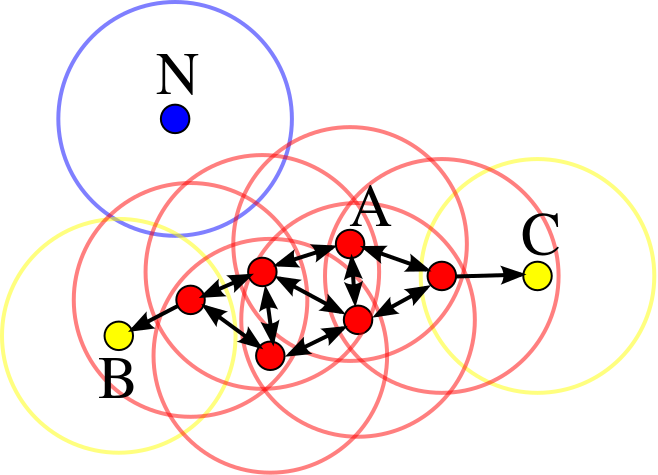
\includegraphics[scale=.4]{DBSCAN.png}
\caption{Diagrama \textbf{DBSCAN}}
\end{figure}

En el diagrama, se puede observar que si fijamos la variable $minPts$ a 3, el punto $A$ y los dem\'as puntos rojos son puntos n\'ucleo, ya que al menos est\'an rodeados de $3$ puntos en su vecindario de radio $\varepsilon$. Como son densamente alcanzables unos con otros, forman un cl\'uster. Los puntos $B$ y $C$ no son puntos n\'ucleo, pero s\'i que son alcanzables desde $A$, por lo que tambi\'en pertenecen al cl\'uster. El punto $N$ es calificiado como aislado o \textit{ruido} ya que no es ni punto n\'ucleo ni densamente alcanzable. \\

La alcanzabilidad no es una relaci\'on sim\'etrica ya que, por definici\'on, ningu\'un punto puede ser alcanzable por un punto no n\'ucleo (un punto no n\'ucleo puede ser alcanzable, pero no puedo \textit{alcanzar}). Es necesario definir una noci\'on m\'as fuerte de \textit{conectividad}. Decimos que $p$ y $q$ est\'an densamente conectados si existe un punto $o$ tal que $p$ y $q$ son densamente alcanzables. Esta noci\'on de \textit{densamente conectados} s\'i que es sim\'etrica.\\

Redefinimos la noci\'on de cl\'uster que previamente hab\'iamos definido. Un cl\'uster debe satisfacer dos propiedades:\\

\begin{enumerate}
	\item Todos los puntos deben estar mutuamente \textit{densamente conectados}.
	\item Si un punto $q$ es densamente alcanzable desde un punto $p$ del cl\'uster, $q$ es parte del cl\'uster tambi\'en. 
\end{enumerate}

\textbf{DBSCAN} requiere de dos par\'ametros para empezar: $\varepsilon$ para la noci\'on de vecindario y $minPts$ para el n\'umero m\'inimo de puntos necesario para formar un cl\'uster. Se empieza tomando arbirariamente un punto del conjunto que no haya sido visitado. Se obtiene su vecindario, en el caso de que no exista, este punto se marca como ruido y se pasa al siguiente. Si no es nulo y tiene un n\'umero de puntos mayor que $minPts$, se crea un cl\'uster. \\

Si uno de los puntos del proceso resulta que es parte de un cl\'uster, su vecindario tambi\'en se a\~nade a \'este. Se reitera este proceso, ya que todos los puntos nuevos a\~nadidos del vecindario anterior, son parte del cl\'uster, luego el vecindario de cada uno es a\~nadido. Este proceso se contin\'ua hasta que se obtiene el cl\'uster densamente conectado. \\

\begin{algorithm}[H]\label{DBSCAN}
\begin{algorithmic}[1]
\Function{DBSCAN}{$positions, eps, minPts$}
	\State{C = 0}
	\For{\textbf{each} pos in positions}
		\If{$pos$ has been visited}
			\State{Continue next position}
		\Else
			\State{Mark $pos$ as visited}
			\State{N(pos) = NeighborPts(pos, eps)}
			\If{$length(N(pos)) < MinPts$}
				\State{Mark $pos$ as noise}
			\Else
				\State{C = next Cluster}
				\State{expandCluster(pos, N(pos), C, eps, MinPts)}				
			\EndIf
		
		\EndIf
	\EndFor
\EndFunction
\State{}
\Function{expandCluster}{$P, NeighborPts, C, eps, MinPts$}
	\State{add P to cluster C}
	\For{\textbf{each} P' in NeighborPts}
		\If{P' is not visited}
			\State{Mark P' as visited}
			\State{NeighborPts' = regionQuery(P', eps)}
			\If{$length(NeighborPts') >= MinPts$}
				\State{NeighborPts = NeighborPts joined with NeighborPts'}
			\EndIf
		\EndIf
		\If{P' is not yet member of any cluster}
			\State{add P' to Cluster C}
		\EndIf
	\EndFor
\EndFunction
\State{}
\Function{NeighborPts}{$P, eps$}
	\State{return all points within P's eps-neighborhood (also P)}
\EndFunction
\end{algorithmic}
\caption{\label{alg:DBSCAN} Algoritmo DBSCAN}
\end{algorithm}

\subsubsection{Implementaci\'on en Python}

Se encuentra una implementaci\'on bastante eficaz y sencilla en el repositorio de \href{https://github.com/SushantKafle/DBSCAN}{Sushant Kafle} \cite{dbscanPython}.\\

\begin{figure}[H]
\begin{python}
from dbscanner import dbscanner
from algorithms.db import connect_db

cur= connect_db("bahia")
recurso = "tetra:12082781"
limit = 1000
cmd = "SELECT latitud, longitud 
	   FROM posicionesgps 
	   WHERE latitud <> 0 and longitud <> 0 
	   AND recurso=\"{0}\" 
	   LIMIT {1};".format(recurso, limit)
cur.execute(cmd)

a=[]
for pos in cur.fetchall():
    a.append([pos[0], pos[1]])

Data = a
eps = 0.0001
MinPts= 5

dbc = dbscanner()
dbc.dbscan(Data, eps, MinPts)
\end{python}
\caption{Ejemplo de uso de la implementaci\'on de \textbf{DBSCAN}}
\end{figure}
\bigskip
Notar que hemos tomado como valor de $\varepsilon = 0.0001$ ya que es una aproximaci\'on de la distancia media de toma entre posiciones y $5$ es un buen valor a la hora de hacer una consolidaci\'on. El resultado consiste en algunas posiciones marcadas como ruido y $5$ cl\'usters. Debido a que es un proceso muy costoso, nos hemos limitado en este caso a hacer la consolidaci\'on en unas $1000$ posiciones.\\

\begin{figure}[H]
	\begin{center}
	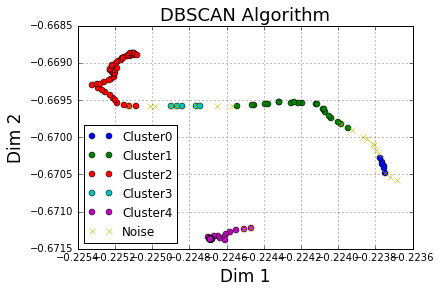
\includegraphics[scale=.7]{dbscan_2_0.png}
	\end{center}
	\caption{Resultado \textbf{DBSCAN}}
\end{figure}

%%%%%%%%%%%%%%%%%%%%%%%%%%%%%%%%%%%%%%%%%%%%%%%%%%%%%%%%%%%%%%%%%%%%%%%%%%%%%%%%%
%%%%%%%%%%%%%%%%%%%%%%%%%%%%%%%%%%%%%%%%%%%%%%%%%%%%%%%%%%%%%%%%%%%%%%%%%%%%%%%%%

\subsection{DJ-Cluster}

\textbf{Density-Joinable Cl\'uster}\cite{importantPlaces} es un tipo de algoritmo de \textit{clustering} basado en densidades de puntos que intenta solventar algunas de las limitaciones de \textbf{K-means}. Este algoritmo localiza puntos significativos sobre el conjunto de todos los puntos, es decir, el centro del cl\'uster. No debemos olvidar que nuestro objetivo es encontrar posiciones significativas en todo nuestro conjunto de posiciones GPS, y \'estos centros de cl\'uster que nos generar\'a este algoritmo nos servir\'an para tal prop\'osito. \\

La idea del algoritmo es la siguiente, para cada punto calculamos su vecindario. Este vecindario depender\'a de la distancia elegida entre todas las anteriores definidas, y seg\'un cu\'al sea la elegida, depender\'a de una variable $\varepsilon$ o un instante $t_0$ escogido. Se impone la condici\'on de que el n\'umero de puntos conseguido al computar su vecindario sea al menos un \textit{MinPts} definido previamente. Si esta condici\'on no se cumple, se marca la posici\'on actual como \textit{ruido} y se prosigue con la siguiente. En el caso de cumplirse, este nuevo punto es el centro del cl\'uster, junto a su vecindario.  \\

Con este nuevo cl\'uster creado, el siguiente paso es comprobar que este cl\'uster no sea \textit{densamente acoplable} con los que ya llevamos computados. Un cl\'uster es \textit{densamente acoplable} a otro cl\'uster si existe un punto com\'un entre ambos. \\

\begin{figure}[H]
\centering
	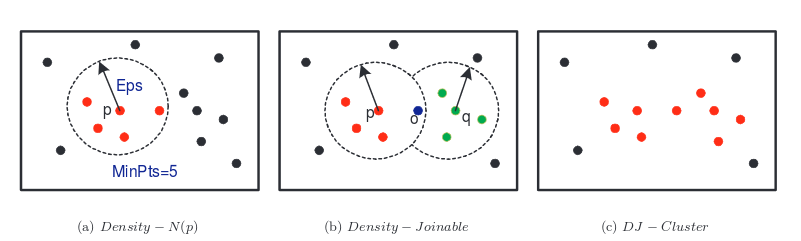
\includegraphics[scale=.7]{djcluster.png}
\caption{Diagrama \textbf{DJ-Clustering}}
\end{figure}

\begin{algorithm}[!htbp]\label{djCluster}
\begin{algorithmic}[1]
	\For{\textbf{each} $p$ in set $S$}
		\State{Compute neighborhood $N(p)$ for $\varepsilon$ and $MinPts$}
		\If{$N(p)$ is null ($|N(p)| < MinPts$ for $\varepsilon$)}
			\State{Label $p$ as noise}
		\ElsIf{$N(p)$ is density-joinable to an existing cluster} 
			\State{Merge $N(p)$ with the cluster which is density-joinable}
		\Else
			\State{Create a new cluster $C$ based on $N(p)$}
		\EndIf
	\EndFor
\end{algorithmic}
\caption{\label{alg:djcluster} Algoritmo DJ-Cluster}
\end{algorithm}

Durante el proceso, se recorren todos los puntos del conjunto a analizar, calculando cada vecindario de cada punto con un centro $p$ y un radio $\varepsilon$. Si el n\'umero de puntos del vecindario excede esta cantidad m\'inima $MinPts$, entonces es un vecindario a considerar. Este cl\'uster es posteriormente \textit{mergeado} con otros posibles cl\'usters densamente acoplables. \\

Al final de cada iteraci\'on puede ser que el n\'umero de cl\'usters no cambie, porque no existe un nuevo cl\'uster o porque el nuevo cl\'uster sea mergeado con alguno de los ya existentes.\\

El valor de los par\'ametros $\varepsilon$ y $MinPts$ es el que determina el tama\~no de nuestros clusters. En nuestro caso, no buscamos grandes n\'umeros de cl\'usters, sino perder el m\'inimo de informaci\'on posible, por lo que nos convendr\'ia tomar unos valores de $\varepsilon$ y $MinPts$ peque\~nos \cite{clusteringApproach}.\\

El valor de la variable $\varepsilon$ debe tomarse\cite{clusteringApproach} en funci\'on de la precisi\'on de los aparatos que toman las posiciones. Podemos estimar este par\'amero por unos $20$ metros, que es la precisi\'on de un GPS convencional. \\

Con respecto al valor de $MinPts$, un valor alto de esta par\'ametro implica que los clusters deben ser m\'as densos a la hora de formarse, pero un valor razonable\cite{clusteringApproach} estar\'ia entre $3$ y $10$.\\

La complejidad de este algoritmo es $\mathcal{O}(n\log{}n)$ \cite{importantPlaces}.\\

En los pr\'oximos resultados utilizaremos una implementaci\'on en Weka para lanzar un estudio, sin embargo, se ha desarrollado en Python el algoritmo de \textbf{DJ-Cl\'uster} de manera parecida al de \textbf{DBSCAN}. Se puede consultar una implementaci\'on en el anexo \ref{App:AppendixB}.


\pagebreak
\section{Aplicaci\'on de los algoritmos}


Se va a realizar una comparativo de todos los m\'etodos estudiados para dos sujetos en concreto de nuestra base de datos. Se han tomado los dos sujetos como m\'as posiciones, y de cada uno de \'estos, un muestreo de $2000$ posiciones. \\

Antes de aplicar los m\'etodos, es necesario aplicar un filtro de Normalizaci\'on, dado que de no aplicarlo, la fecha pesar\'ia sobre todos los dem\'as y dejar\'ia el resto de las variables sin valor (no hay que olvidar que la fecha es un \texttt{timestamp}, por lo que a efectos pr\'acticos es un entero muy grande). 

\begin{figure}[H]
	\begin{tabular}{| l | l |}
	\hline
		\textbf{Sujeto 1} & tetra:12082781 \\
		\textbf{Sujeto 2} & tetra:12082364 \\	
	\hline
	\end{tabular}
\end{figure}

Antes de importar las variables de nuestra base de datos, necesitamos hacer el c\'alculo de su media y su desviaci\'on t\'ipica con el fin de tipificar cada una de las variables y dar la misma importancia a cada una de ellas. \\

Para el primer sujeto, contamos con lo siguiente:\\

	\begin{tabular}{l|l|l|l}
	\rowcolor{LightCyan}
	\hline
		& latitud & longitud & fecha\\
	\hline
		Media & -0.223 & -0.665 & 1424174494.89 \\
		Desv. T\'ipica & 0.022 & 0.065	& 104277.37 \\
	\end{tabular}
	
\bigskip

Hacemos una importaci\'on de datos a Weka de la siguiente forma:\\

\begin{lstlisting}[language=sql, columns=fullflexible, basicstyle=\small, frame=tblr]
mysql > SELECT (latitud + 0.223)/0.022 as 'latitudT', 
	(longitud + 0.665)/0.065 as 'longitudT',
	(UNIX_TIMESTAMP(fecha) - 1424174494.89)/104277.37 as 'time'
	FROM posicionesgps
	WHERE latitud <> 0 AND longitud <> 0 
		AND recurso='tetra:12082781'
	LIMIT 2000;
\end{lstlisting}

\begin{figure}[H]
	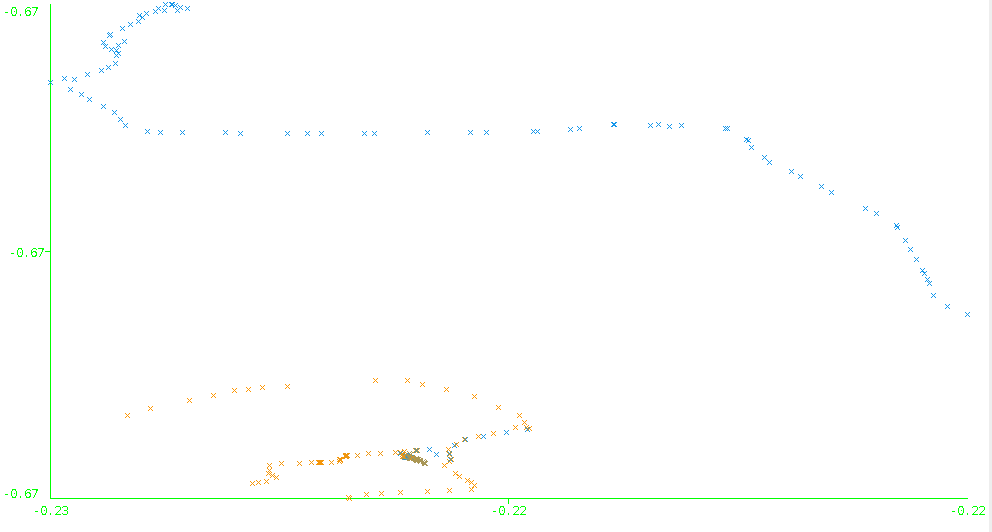
\includegraphics[scale=.5]{../comparativa/sujeto1.png}
	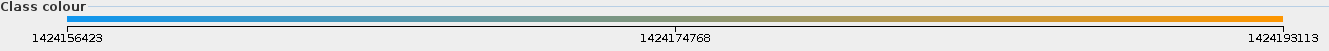
\includegraphics[scale=.4]{../comparativa/leyenda.png}
	\caption{Distribuci\'on de las 2.000 posiciones del Sujeto 1}
\end{figure}

Se hace una distinci\'on de colores azules y naranjas en funci\'on del tiempo. Se puede observar la traza de movimiento del sujeto, que empieza en la esquina superior izquierda y acaba en la parte inferior de la gr\'afica. \\

Calculamos la desviaci\'on t\'ipica y la media del segundo sujeto, del mismo modo que con el sujeto 1.\\

	\begin{tabular}{l|l|l|l}
	\rowcolor{LightCyan}
		& latitud & longitud & fecha\\
	\hline
		Media & -0.21 & -0.625 & 1424350386.203 \\
		Desv. T\'ipica & 0.057 & 0.169 & 41234.453 \\
	\end{tabular}

	
	\bigskip

Para el segundo sujeto, hacemos una importaci\'on de datos a partir de nuestra base de datos de la siguiente forma:\\

\begin{lstlisting}[language=sql, columns=fullflexible, basicstyle=\small, frame=tblr]
mysql > SELECT (latitud + 0.21)/0.057 as 'latitudT', 
(longitud + 0.625)/0.169 as 'longitudT', 
(UNIX_TIMESTAMP(fecha) - 1424350386.203)/41234.453 as 'time'
FROM posicionesgps
WHERE recurso='tetra:12082364' AND latitud<>0 AND longitud<>0
ORDER BY 3 ASC
LIMIT 2000;
\end{lstlisting}

\begin{figure}[H]
	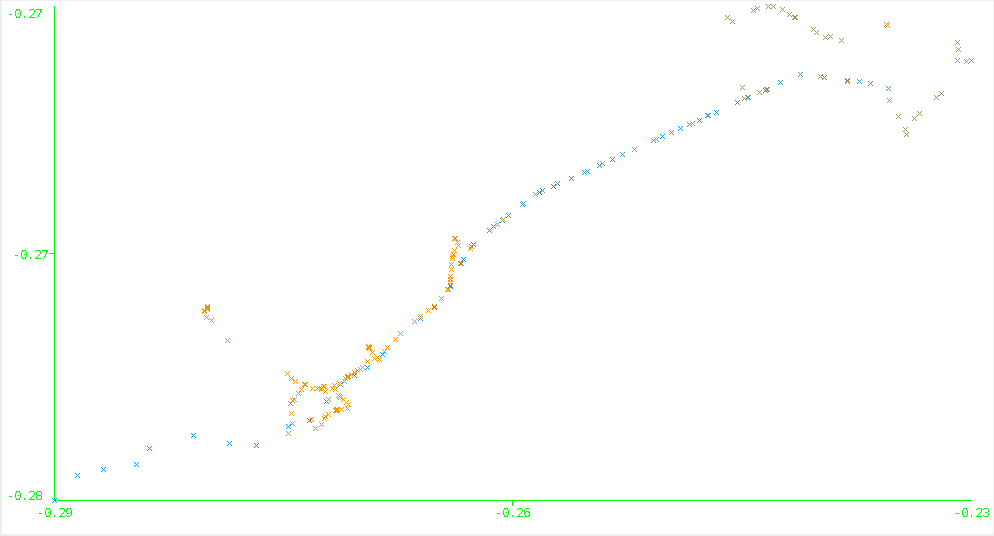
\includegraphics[scale=.5]{../comparativa/sujeto2.png}
	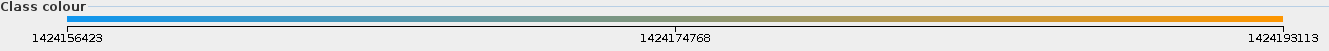
\includegraphics[scale=.4]{../comparativa/leyenda.png}
	\caption{Distribuci\'on de las 2.000 posiciones del Sujeto 2}
\end{figure}

\subsection{Resultados de algoritmos por consolidaci\'on simple}

La importaci\'on de datos para poder utilizar los algoritmos que se han desarrollado en la secci\'on \ref{sec:simple} es parecida a la utilizada en el algoritmo \textbf{DBSCAN}.\\ 

Utilizaremos la clase \texttt{db} que hemos creado para conectarnos a la base de datos donde almacenamos las posiciones:\\

\begin{python}
cur_sal = connect_db("bahia")
limit = 2000
cmd = "SELECT * FROM posicionesgps WHERE latitud<>0 
			AND longitud<> 0 AND recurso='tetra:12082781' 
			LIMIT {0};".format(limit)
cur_sal.execute(cmd)
\end{python}

\bigskip
Y crearemos una lista de posiciones con la implementaci\'on previa que hemos desarrollado:\\

\begin{python}
list_pos = []
for row in cur_sal.fetchall():
	q = Position(row[0] # id
		, row[2] # resource
		, row[3] # lat
		, row[4] # lon
		, row[5] # speed
		, row[6] # track
		, row[10] # date
		)
	list_pos.append(q)
\end{python}

\smallskip
Tipificaremos las variables como anteriormente hemos hecho, calculando su media y su desviaci\'on t\'ipica:\\

\begin{python}
listPosTyp = []
lats = []
longs = []

for pos in list_pos:
    lats.append(pos.lat)
meanLat = np.mean(lats)
for pos in list_pos:
    longs.append(pos.lon)
meanLon = np.mean(longs)
devLat = np.std(lats)
devLon = np.std(longs)

latsTyp = []
longsTyp = []
for pos in list_pos:
	q = Position(pos.id, pos.resource
	, (pos.lat - meanLat)/devLat
	, (pos.lon - meanLon)/devLon
	, pos.speed, pos.track, pos.date)
	listPosTyp.append(q)
	latsTyp.append(q.lat)
	longsTyp.append(q.lon)
\end{python}

\bigskip
Utilizaremos el c\'odigo definido en el anexo \ref{App:AppendixB} para realizar las consolidaciones por adelgazamiento, tiempo y distancia.\\

\begin{python}
import consolidation as cs
\end{python}

\pagebreak
\subsubsection{Consolidaci\'on por adelgazamiento}

Y vamos a realizar una primera consolidaci\'on por adelgazamiento, se mantienen 2 posiciones de cada 5:\\

\begin{python}
result = cs.ConsolidationByThinning(list_pos, 2, 5)
\end{python}

\bigskip

Utilizando \texttt{matplotlib}, dibujamos los resultados.\\

\begin{figure}[H]
	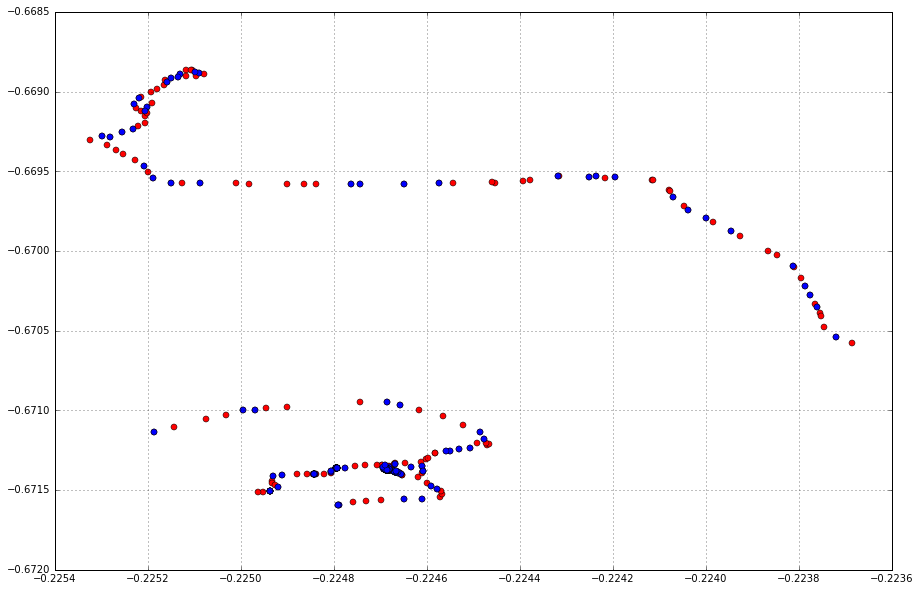
\includegraphics[scale=.45]{../comparativa/thinningSuj1.png}
	\caption{Resultado consolidaci\'on por adelgazamiento}
\end{figure}

Los puntos rojos son los eliminados porque se han consolidado y los azules son los que se han mantenido. En este caso, se mantienen 800 posiciones. \\

\pagebreak
\subsubsection{Consolidaci\'on por tiempo}

Realizaremos una consolidaci\'on por tiempo, eliminaremos las posiciones que tengan entre ellas un lapso menor que $20$:\\

\begin{python}
result = cs.ConsolidationByTime(list_pos, 20)
\end{python}

\begin{figure}[H]
	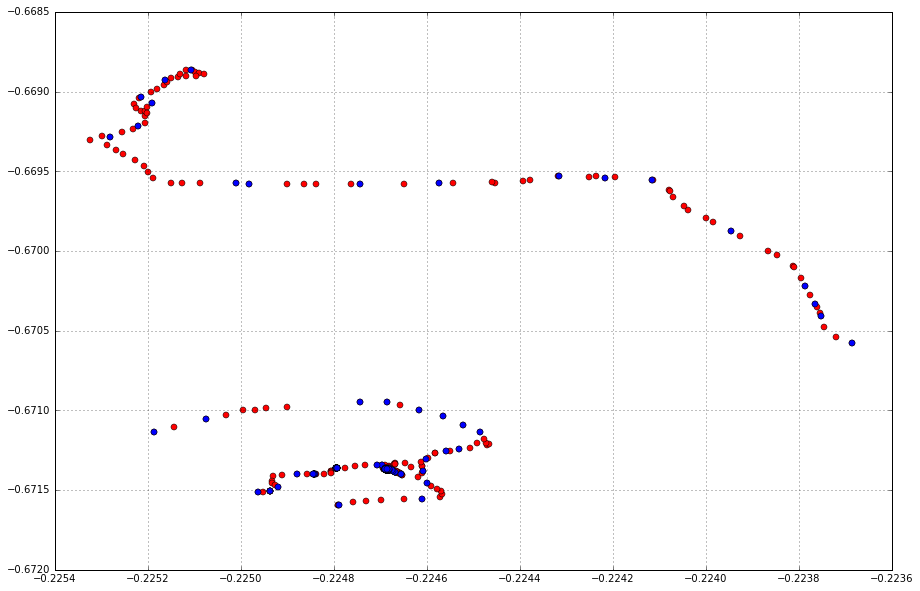
\includegraphics[scale=.45]{../comparativa/byTimeSuj1.png}
	\caption{Resultado consolidaci\'on por tiempo}
\end{figure}

En este caso se mantienen 507 posiciones.

\pagebreak
\subsubsection{Consolidaci\'on por distancia simple}

Se realiza una consolidaci\'on por distancia simple, es decir, por distancia eucl\'idea dando un radio de $\varepsilon = 0.0001$:\\

\begin{python}
result = cs.ConsolidationByDistance(list_pos, 0, 0.0001, 1)
\end{python}

\begin{figure}[H]
	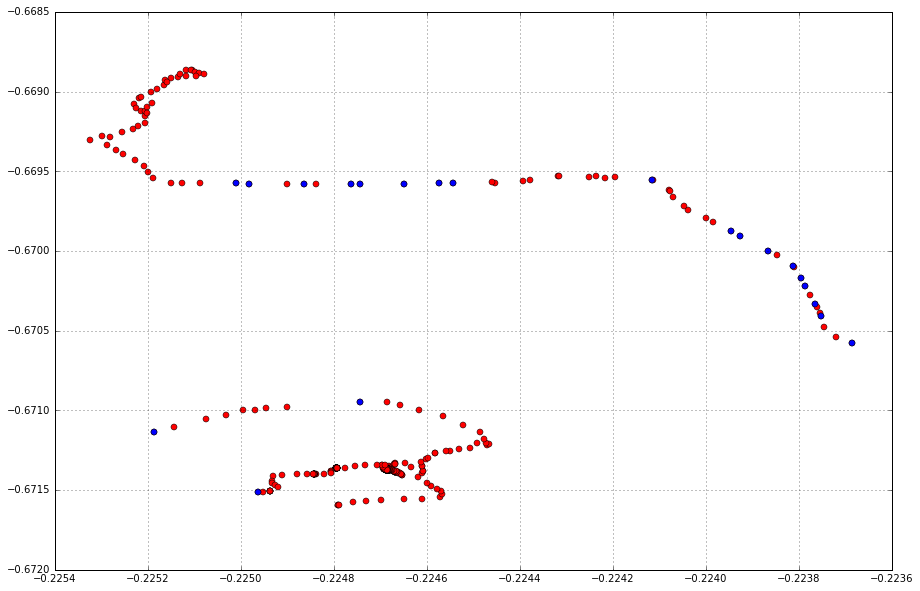
\includegraphics[scale=.45]{../comparativa/distanceEuEps10-4.png}
	\caption{Resultado consolidaci\'on por distancia Simple}
\end{figure}

Se han reducido el n\'umero de puntos a 21.\\

\subsubsection{Consolidaci\'on por distancia t0-alcanzable}

\begin{python}
cs.ConsolidationByDistance(list_pos, 2, 0.001, 1)
\end{python}

\begin{figure}[H]
	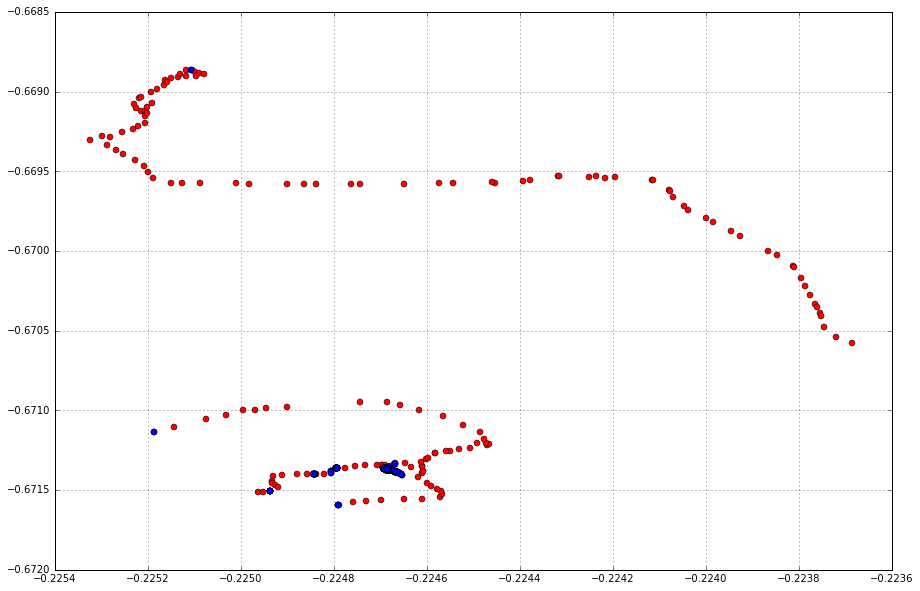
\includegraphics[scale=.45]{../comparativa/t0Sujet1.png}
	\caption{Resultado consolidaci\'on por distancia $t_0-$alcanzable}
\end{figure}

Esta consolidaci\'on, que tiene en cuenta la velocidad instant\'anea del sujeto, realiza una consolidaci\'on m\'as severa en aquellos puntos en los cuales el sujeto posee velocidad, es decir, el vecindario de \'estos puntos es superior al vecindario de los puntos donde no posee velocidad. Esta es la raz\'on por la cual la traza superior (en la que el sujeto tiene una mayor velocidad) ha sido consolidada s\'olo al punto inicial. \\

Esta consolidaci\'on ha mantenido 1786 puntos.\\

\pagebreak
\subsection{Resultados con K-means}

Se va a realizar un estudio \textbf{K-means} para ambos sujetos con los mismos par\'ametros que previamente hab\'iamos aplicado, vamos a reducir el n\'umero de posiciones a $500$, es decir, una consolidaci\'on al $25\%$. En ambos experimentos se ha tomado una distancia eucl\'idea por simplicidad. Se aplicar\'a un preprocesado de \textit{Canopy} y fijaremos el n\'umero de cl\'usters a $500$: \\

\subsubsection{Sujeto 1}

\begin{verbatim}
=== Run information ===

Scheme:       weka.clusterers.SimpleKMeans -init 2 -max-candidates 100 
				-periodic-pruning 10000 -min-density 2.0 
				-t1 -1.25 -t2 -1.0 -N 500 -A "weka.core.EuclideanDistance 
				-R first-last" -I 500 -num-slots 1 -S 10
Relation:     QueryResult
Instances:    2000
Attributes:   3
              latitudT
              longitudT
              time
Test mode:    evaluate on training data


=== Clustering model (full training set) ===


kMeans
======

Number of iterations: 9
Within cluster sum of squared errors: 0.11736312393686821

Initial starting points (canopy):

T2 radius: 0,504     
T1 radius: 0,631  

Cluster 0: -0.077067,-0.09795,0.073287
Cluster 1: -0.076555,-0.097964,-0.092632
Cluster 2: -0.044869,-0.075594, -0.166324
...

Time taken to build model (full training data) : 0.69 seconds
\end{verbatim}


\begin{figure}[H]
	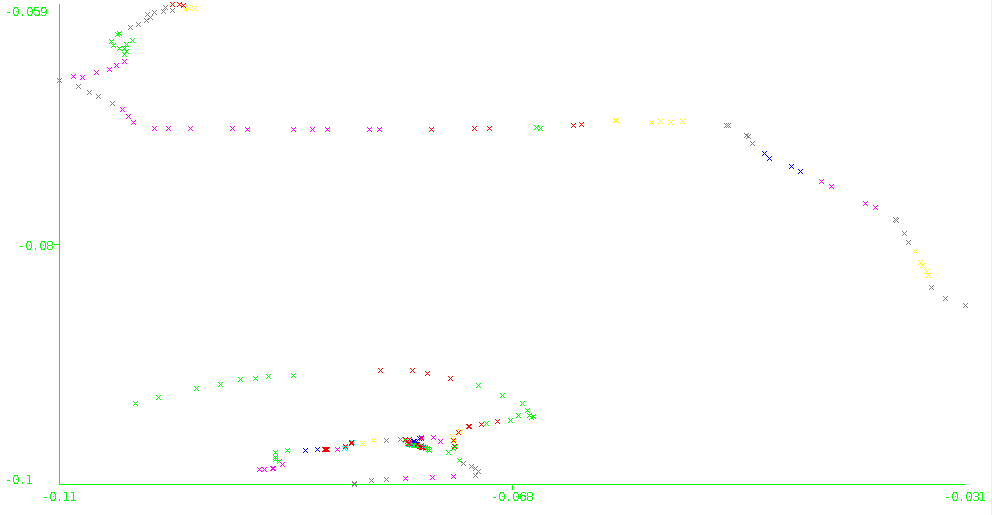
\includegraphics[scale=.5]{../comparativa/kMeansSujeto1.png}
	\caption{Resultado de \textbf{K-means} para el Sujeto 1}
\end{figure}

Se han realizado $10$ iteraciones y se ha llegado a un error cuadr\'atico de $0.117363$. Observando el n\'umero de posiciones que ha agrupado por cl\'uster, podemos observar que var\'ian entre $1$ y $9$, lo cual es una buena media, ya que no ha agrupado demasiadas posiciones en un mismo cl\'uster. Debemos recordar que nuestro objetivo no es conseguir una cantidad de cl\'usters muy peque\~na, sino conseguir que cada cl\'uster cuente con un n\'umero m\'as o menos equilibrado de posiciones, para poder asignar cada posici\'on a su centro del cl\'uster.\\ 

Se puede observar mejor en la gr\'afica. Cada cl\'uster est\'a representado por un color distinto. En la parte superior de esta gr\'afica, podemos observar que ha seguido un camino con respecto al tiempo en una direcci\'on, mientras que en la parte inferior ha pasado varias veces por un mismo sitio, y aparece una aglomeraci\'on de colores en un punto. Esto se debe a que para nuestro estudio hemos introducido tambi\'en la variable temporal, por lo que no puede agrupar todas esas posiciones en un mismo cl\'uster, ya que no lo est\'an, debido a que vienen de varios instantes distintos. \\

El total de cl\'usters es de 500, ya que con \textbf{K-means} es necesario prefijarlos.


\subsubsection{Sujeto 2}

Realizamos el mismo estudio con el Sujeto 2:\\

\begin{verbatim}
=== Run information ===

Scheme:       weka.clusterers.SimpleKMeans -init 2 -max-candidates 500 
						-periodic-pruning 10000 -min-density 2.0 
						-t1 -1.25 -t2 -1.0 -N 500 
						-A "weka.core.EuclideanDistance -R first-last" 
						-I 500 -num-slots 1 -S 10
Relation:     QueryResult
Instances:    2000
Attributes:   3
              latitudT
              longitudT
              time
Test mode:    evaluate on training data


=== Clustering model (full training set) ===


kMeans
======

Number of iterations: 24
Within cluster sum of squared errors: 0.2079975699953984

Initial starting points (canopy):

T2 radius: 0,439     
T1 radius: 0,548     

Cluster 0: -0.278213,-0.272406,0.032468,
Cluster 1: -0.236123,-0.267776,-0.148367
......

Time taken to build model (full training data) : 1.38 seconds
\end{verbatim}


\begin{figure}[H]
	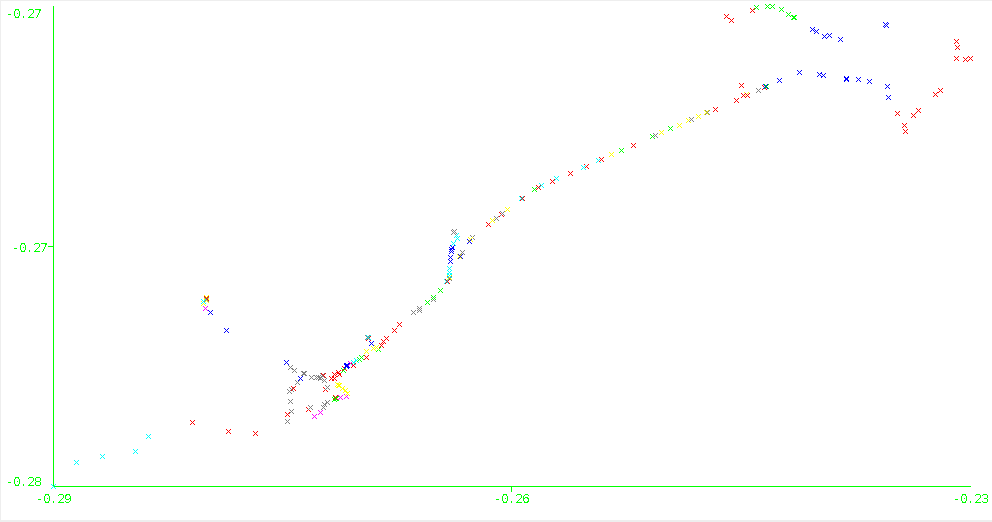
\includegraphics[scale=.5]{../comparativa/kMeansSujeto2.png}
	\caption{Resultado de \textbf{K-means} para el Sujeto 1}
\end{figure}

En la siguiente figura, se observa una asignaci\'on un poco rara de los cl\'usters. En la secci\'on de abajo se pueden observar distintos colores, como si varios puntos muy cercanos se hubieran asingados a cl\'usteres distintos, pero esto es debido a que no son seguidos en el tiempo, es decir, el sujeto est\'a volviendo a pasar por el mismo sitio. Si nos volvemos a fijar en la representaci\'on sin clusterizar, se puede observar que existe un trozo donde el naranja y el azul se superponen, es decir, son instantes distantes temporalmente.\\

El error cuadr\'atico es de $0.207997$, un poco peor que con el sujeto 1, y el tiempo de ejecuci\'on es de $1.38$ segundos.\\

\pagebreak
\subsection{Resultados con DBSCAN}

Utilizaremos los mismos par\'ametros utilizados para el m\'etodo \textbf{DBSCAN} previamente estudiado, un valor de $\varepsilon = 0.0001$ y un valor de $minPts = 5$. Tomaremos $1000$ datos de cada sujeto y los compararemos:\\

\subsubsection{Sujeto 1}

\begin{python}
cur= connect_db("bahia")
recurso = "tetra:12086044"
limit = 2000
cmd = "SELECT latitud, longitud, UNIX_TIMESTAMP(fecha) 
	FROM posicionesgps 
	WHERE latitud <> 0 and longitud <> 0 and recurso=\"{0}\" 
	LIMIT {1};".format(recurso, limit)
cur.execute(cmd)

a=[]
for pos in cur.fetchall():
    a.append([pos[0], pos[1], pos[2]])

Data = a
eps = 0.0001
MinPts=5

dbc = dbscanner()
dbc.dbscan(Data, eps, MinPts)
\end{python}

\bigskip

Una de las cosas positivas que se puede decir del algoritmo \textbf{DBSCAN} es que identifica puntos como \textit{ruido}, cosa que los algoritmos de \textbf{K-means} y \textbf{DJ-Cluster} no hacen, ya que asignan simplemente esos puntos a un cl\'uster de un \'unico punto.\\

El resultado de DBSCAN ha sido una divisi\'on de nuestro conjunto inicial de $1000$ posiciones en 6 cl\'usters y algunas posiciones etiquetadas como ruido.


\begin{figure}[H]
	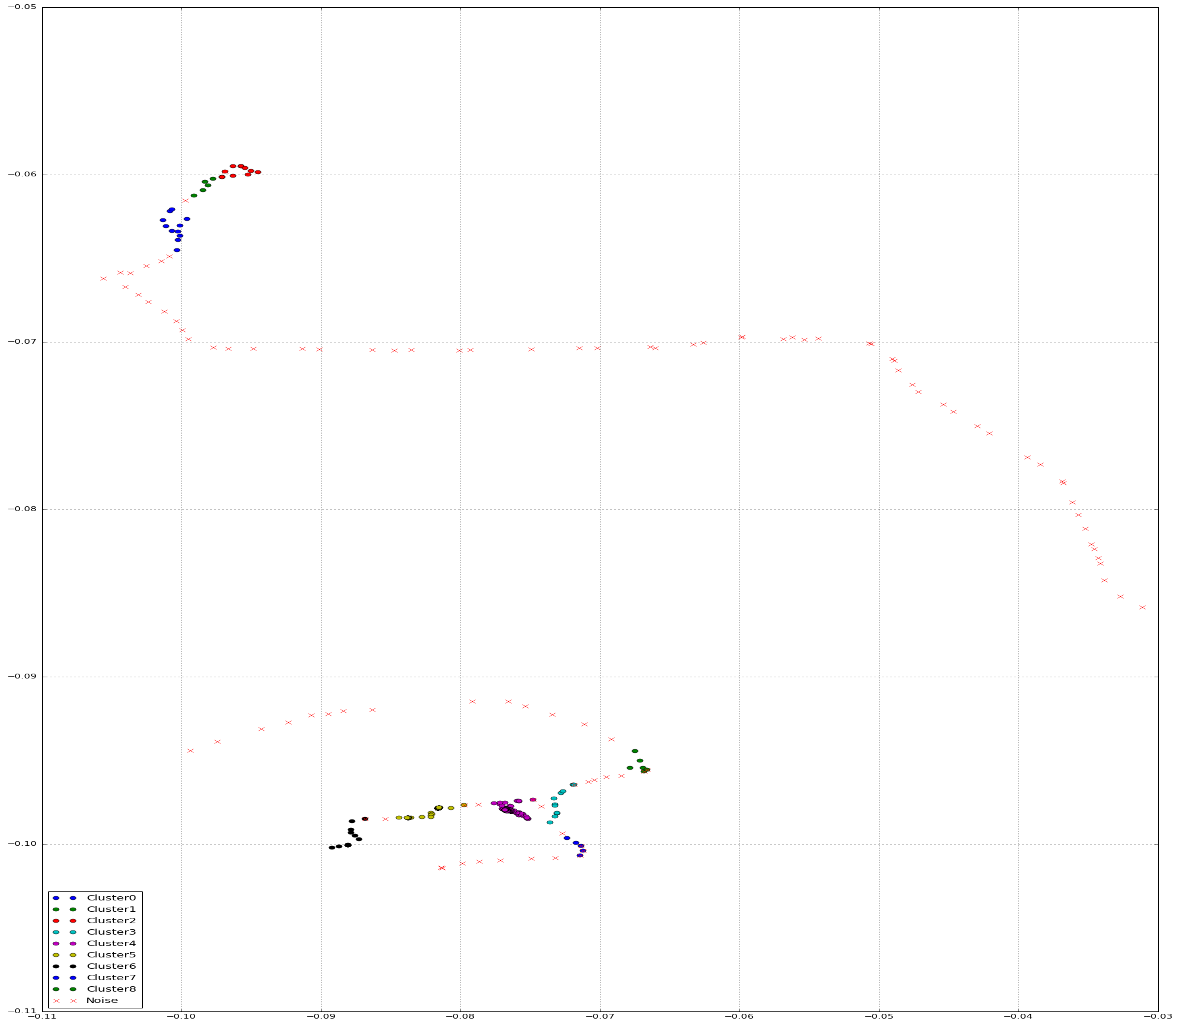
\includegraphics[width=15cm]{../comparativa/dbscanSujeto1.png}
	\caption{Resultado de \textbf{DBSCAN} para el Sujeto 1}
\end{figure}


\subsubsection{Sujeto 2}

Utilizaremos los mismos par\'ametros utilizados para el sujeto 1:\\

\begin{python}
cur= connect_db("bahia")
recurso = "tetra:12082781"
limit = 2000
cmd = "SELECT latitud, longitud, UNIX_TIMESTAMP(fecha) 
	FROM posicionesgps 
	WHERE latitud <> 0 and longitud <> 0 and recurso=\"{0}\" 
	LIMIT {1};".format(recurso, limit)
cur.execute(cmd)

a=[]
for pos in cur.fetchall():
    a.append([pos[0], pos[1], pos[2]])

Data = a
eps = 0.0001
MinPts=5

dbc = dbscanner()
dbc.dbscan(Data, eps, MinPts)
\end{python}

\begin{figure}[H]
	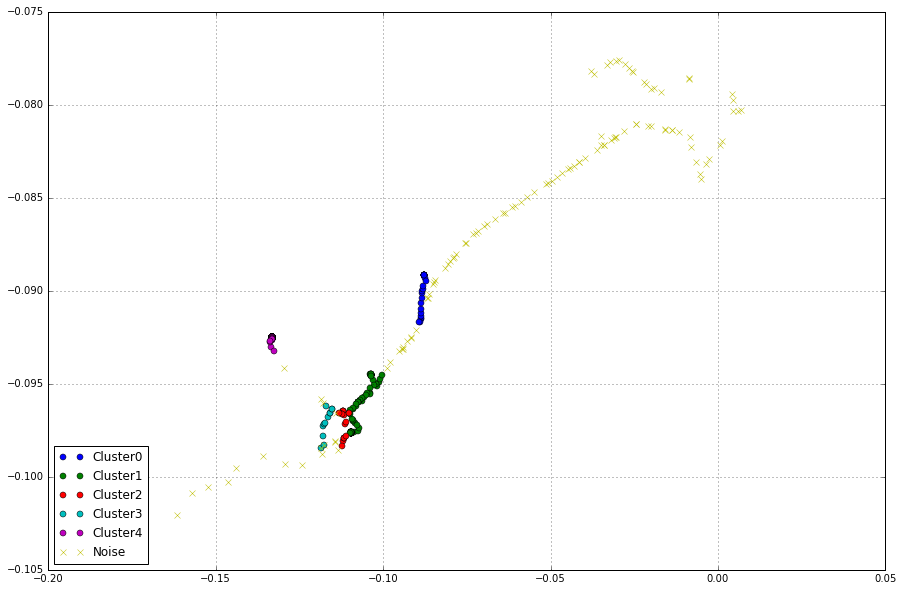
\includegraphics[width=15cm]{../comparativa/dbscanSujeto2.png}
	\caption{Resultado de \textbf{DBSCAN} para el Sujeto 2}
\end{figure}

Obtenemos 5 cl\'usters en un tiempo de ejecuci\'on de 2 minutos, 20 segundos. En esta ejecucci\'on, ha etiquetado muchas posiciones como ruido, probablemente son las posiciones en las cuales el sujeto se encuentra en movimiento. De haber utilizado aqu\'i una consolidaci\'on en la cual se hubiera introducido una distancia que involucrara la velocidad, habr\'iamos consolidado en esa zona superior derecha de ruido un nuevo cl\'uster. \\

Haciendo un peque\~no cambio en el c\'odigo que podemos encontrar de la implementaci\'on de DBSCAN en el ap\'endice \ref{App:AppendixB}.\\

\pagebreak

\begin{python}
def regionQuery(self,P,eps):
	P = Position(None, None, P.X, P.Y, P.Speed, None, None)
	for d in self.dataSet:
		d = Position(None, none, d.X, d.Y, d.Speed, None, None)
		if d.is_in_neighborhoodByEURelativeSpeed(P, 0.001):
			result.append(d)
	return result
\end{python}

As\'i estar\'iamos utilizando la distancia que hemos implementado que involucra la velocidad.

\subsection{Resultados con DJ-Cluster}

Realizaremos un estudio \textbf{DJ-Cluster} utilizando un preprocesado de datos \textbf{Canopy} fijando una desviaci\'on m\'inima est\'andar de $0.001$. \\

Se fija una distancia eucl\'idea para ambos experimentos.\\

\subsubsection{Sujeto 1}

Notar que si utilizamos un preprocesado de \textit{Canopy} sin fijar el n\'umero de cl\'usters previo, \'este nos consolida demasiado la informaci\'on (tal y como pasa en el DBSCAN), lo cual no es muy interesante.\\

\begin{verbatim}
=== Run information ===

Scheme:       weka.clusterers.MakeDensityBasedClusterer -M 0.001 
						-W weka.clusterers.Canopy -- 
						-N -1 -max-candidates 100 
						-periodic-pruning 10000 
						-min-density 2.0 -t2 -1.0 -t1 -1.25 -S 1
Relation:     QueryResult
Instances:    2000
Attributes:   3
              latitudT
              longitudT
              time
Test mode:    evaluate on training data


=== Clustering model (full training set) ===

MakeDensityBasedClusterer: 

Wrapped clusterer: 
Canopy clustering
=================

Number of canopies (cluster centers) found: 4
T2 radius: 0,504     
T1 radius: 0,631     

Cluster 0: -0.094874,-0.065178,-0.166183,{55} <0>
Cluster 1: -0.076573,-0.097976,-0.028496,{1474} <1,2>
Cluster 2: -0.077869,-0.097886,0.137391,{438} <1,2>
Cluster 3: -0.044869,-0.075594,-0.166324,{33} <3>

Time taken to build model (full training data) : 0.03 seconds

=== Model and evaluation on training set ===

Clustered Instances

0        51 (  3%)
1      1170 ( 59%)
2       742 ( 37%)
3        37 (  2%)


Log likelihood: 9.34996
\end{verbatim}

\begin{figure}[H]
	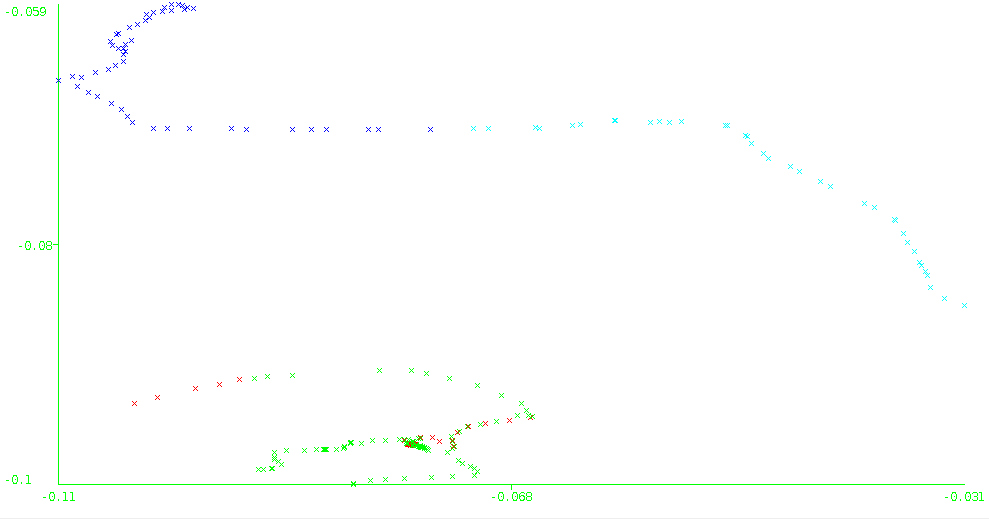
\includegraphics[scale=.5]{../comparativa/djClusterPruebaCanopySin.png}
	\caption{Resultado de \textbf{DBSCAN} para el Sujeto 2}
\end{figure}


Realizaremos un preprocesado \textit{Canopy} de $500$ cl\'usters, con el fin de conseguir \textit{tanta} consolidaci\'on.\\

\begin{verbatim}
=== Run information ===

Scheme:       weka.clusterers.MakeDensityBasedClusterer -M 0.001 
					-W weka.clusterers.Canopy -- 
					-N 500 -max-candidates 100 
					-periodic-pruning 10000 
					-min-density 2.0 -t2 -1.0 -t1 -1.25 -S 1
Relation:     QueryResult
Instances:    2000
Attributes:   3
              latitudT
              longitudT
              time
Test mode:    evaluate on training data


=== Clustering model (full training set) ===

MakeDensityBasedClusterer: 

Wrapped clusterer: 
Canopy clustering
=================

Number of canopies (cluster centers) found: 500
T2 radius: 0,504     
T1 radius: 0,631     

Cluster 0: -0.094874,-0.065178,-0.166183,
Cluster 1: -0.076573,-0.097976,-0.028496
...
\end{verbatim}

El cual nos consigue un preprocesado de $500$ cl\'usters con Canopy, sin embargo, al aplicar DJ-Cluser, se nos reduce a $22$ cl\'usters:\\

\begin{verbatim}
Time taken to build model (full training data) : 0.37 seconds

=== Model and evaluation on training set ===

Clustered Instances

  0         3 (  0%)
 12       605 ( 30%)
 58         7 (  0%)
142       449 ( 22%)
165         3 (  0%)
209        57 (  3%)
230       188 (  9%)
287         8 (  0%)
295        32 (  2%)
345        17 (  1%)
353         9 (  0%)
369        68 (  3%)
373         3 (  0%)
380         6 (  0%)
385         2 (  0%)
386        10 (  1%)
458         7 (  0%)
459         3 (  0%)
464         3 (  0%)
473         9 (  0%)
474         1 (  0%)
493       510 ( 26%)


Log likelihood: 9.05128
\end{verbatim}


\begin{figure}[H]
	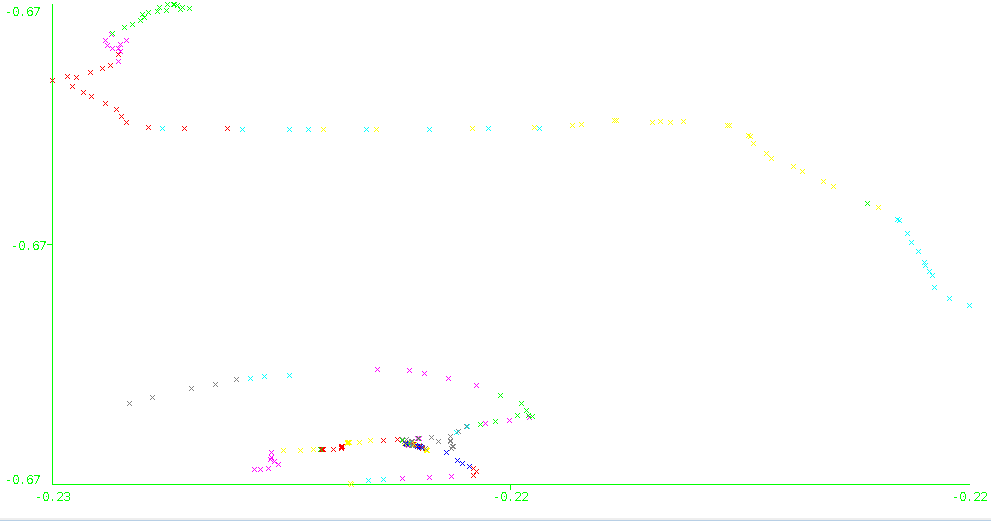
\includegraphics[scale=.5]{../comparativa/djClusterSujeto1.png}
	\caption{Resultado de \textbf{DJ-Cluster} para el Sujeto 1}
\end{figure}

Este resultado se puede interpretar como algo bastante positivo, ya que hemos reducido considerablemente el tama\~no de nuestra base de datos, e incluso podemos etiquetar algunos cl\'usters como ruido, es decir, aquellos que s\'olo se nos han producido a partir de una o dos posiciones como es el caso. Ser\'ia necessario hacer un \textit{post-procesado} de datos para eliminar todas estas posiciones aisladas.

\subsubsection{Sujeto 2}

Con el sujeto 2 ocurre lo mismo que con el sujeto 1, con el preprocesado de \textit{Canopy} obtenemos una consolidaci\'on en $500$ cl\'usters, sin embargo, al aplicar \textbf{DJ-Cluster}, obtenemos una consolidaci\'on a 27 cl\'usters.\\

\begin{verbatim}

Time taken to build model (full training data) : 1.56 seconds


=== Model and evaluation on training set ===

Clustered Instances

  0         6 (  0%)
  2         5 (  0%)
  3         1 (  0%)
  4         2 (  0%)
 76         5 (  0%)
 91         6 (  0%)
 96        36 (  2%)
107         1 (  0%)
133         6 (  0%)
142        91 (  5%)
146        68 (  3%)
159         4 (  0%)
166        19 (  1%)
173         1 (  0%)
211        17 (  1%)
214         2 (  0%)
288         8 (  0%)
329      1669 ( 83%)
354         5 (  0%)
370         1 (  0%)
381         1 (  0%)
386         5 (  0%)
387        10 (  1%)
391         1 (  0%)
459         4 (  0%)
474        16 (  1%)
475        10 (  1%)


Log likelihood: 10.83917
\end{verbatim}

\begin{figure}[H]
	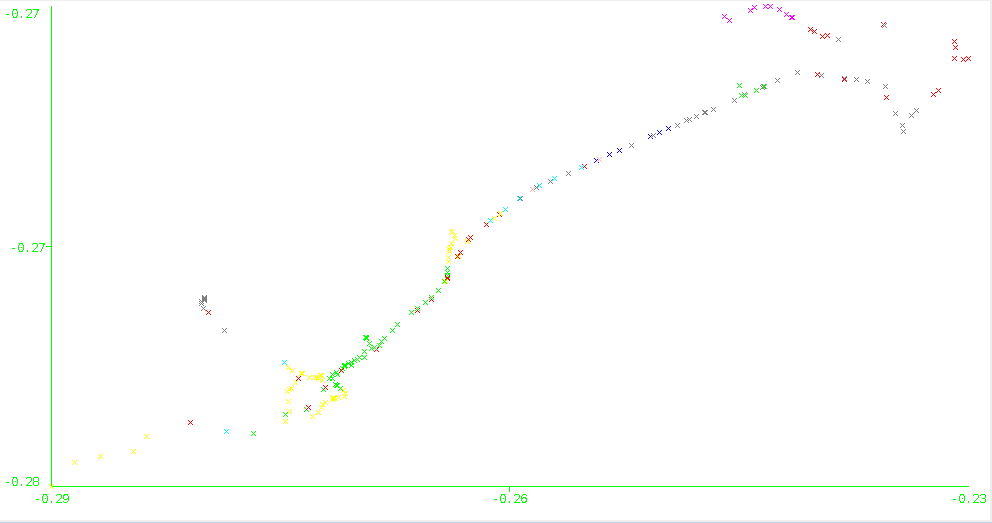
\includegraphics[scale=.5]{../comparativa/djClusterSujeto2.png}
	\caption{Resultado de \textbf{DJ-Cluster} para el Sujeto 2}
\end{figure}


\pagebreak
\section{Comparativa de resultados}

\begin{center}
\begin{figure}[H]
	\begin{tabular}{|p{2.5cm}|l|l|}
	\hline
  		\cellcolor{blue!25}\textbf{Algoritmo} 
  		& \cellcolor{blue!25}\textbf{SUJETO 1} 
  		& \cellcolor{blue!25}\textbf{SUJETO 2} \\
	\hline
	\hline
		K-\textbf{means} & 
		\begin{tabular}{l l}
			Canopy & S\'i\\
			N. Cl\'usters & 500 \\
			Iteraciones & 9 \\
			Error cuadr\'atico & 0.117363 \\
			T. de ejecuci\'on & 0.69 secs
		\end{tabular} &
		\begin{tabular}{l l}
			Canopy & S\'i\\
			N. Cl\'usters & 500 \\
			Iteraciones & 24 \\
			Error cuadr\'atico & 0.208997 \\
			T. de ejecuci\'on & 1.38 secs
		\end{tabular}  \\
		\hline
		\textbf{DBSCAN} & 
		\begin{tabular}{l l}
			Canopy: & No\\
			Iteraciones: & 111 \\
			T. de ejecuci\'on: & 2 min 30 secs\\
			N. Cl\'usters: & 9
		\end{tabular}				
		& \begin{tabular}{l l}
			Canopy: & No\\
			Iteraciones: & 111 \\
			T. de ejecuci\'on: & 2 min 20 secs\\
			N. Cl\'usters: & 9
		\end{tabular} \\
		\hline
		\textbf{DJ-Cl\'uster} & 
		\begin{tabular}{l l}
			Canopy: & S\'i \\
			Iteraciones: & 11\\
			Cl\'usters: & 22\\
			Error cuadr\'atico: & 0.140929\\
			Verosimilitud: & 9.34996	\\
			T. de ejecuci\'on & 0.37 secs
		\end{tabular} & 
		\begin{tabular}{l l}
			Canopy: & S\'i \\
			Iteraciones: & 12\\
			N. Cl\'usters: & 27\\
			Error cuadr\'atico: & 0.209090\\
			Verosimilitud: & 10.83638\\
			T. de ejecuci\'on & 1.56 secs
		\end{tabular}\\
		\hline
		\textbf{Por adelgazamiento} & 
		\begin{tabular}{ll}
			Canopy: & No \\
			Iteraciones: & N. de posiciones \\
			Cl\'usters: & 800\\
			T. de ejecuci\'on: & < 0.01 sec
		\end{tabular} & \\
		\hline
		\textbf{Por tiempo} & 
		\begin{tabular}{ll}
			Canopy: & No \\
			Iteraciones: & N. de posiciones \\
			Cl\'usters: & 507\\
			T. de ejecuci\'on: & < 0.01 sec
		\end{tabular} & \\
		\hline
		\textbf{Por distancia simple} & 
		\begin{tabular}{ll}
			Canopy: & No \\
			Iteraciones: & N. de posiciones \\
			Cl\'usters: & 21\\
			T. de ejecuci\'on: & < 0.01 sec
		\end{tabular} & \\
		\hline
		\textbf{Por distancia $t_0$-alcanzable} & 
		\begin{tabular}{ll}
			Canopy: & No \\
			Iteraciones: & N. de posiciones \\
			Cl\'usters: & 1786\\
			T. de ejecuci\'on: & < 0.01 sec
		\end{tabular} & \\
		\hline
	\end{tabular}
	\caption{Comparativa entre los disintos m\'etodos}
\end{figure}

\end{center}

Se puede observar que claramente el algoritmo \textbf{DBSCAN} es el m\'as lento de todos, adem\'as del que m\'as iteraciones realiza. Sin embargo, \'este es el que menos cl\'usters obtiene, es decir, el que realiza una consolidaci\'on mayor. Esto es debido a que no lleva un preprocesado \textit{Canopy} previo, no como \textbf{K-means} y \textbf{DJ-Cluster}. Ambos llevan un preprocesado previo de \textit{Canopy}, el cual les marca un n\'umero m\'inimo de cl\'usters que dejar a la hora de realizarlo, sin embargo, podemos observar que \textbf{K-means} se queda en los $500$ cl\'usters que le hemos fijado desde el principio, mientras que \textbf{DJ-Cluster} consigue rebajar este n\'umero incluso m\'as. Con respecto al tiempo de ejecuci\'on, \textbf{DJ-Cluster} es much\'isimo m\'as efectivo, aunque su error cuadr\'atico es peor, comparado con \textbf{K-means}.\\

\textbf{DBSCAN} tiene algunas ventajas con respecto a sus dem\'as compa\~neros:

\begin{itemize}
	\item No necesita de prefijar el n\'umero de cl\'usters.
	\item DBSCAN tiene la noci\'on de ruido, as\'i que no es necesario aplicar un post-filtro para encontrar aquellos puntos aislados. 
\end{itemize}

Sin embargo, \textit{DBSCAN} no es un algoritmo determinista, los puntos borde que son alcanzables desde m\'as de un s\'olo cl\'uster pueden asignarse a cualquiera de \'estos. Sin embargo, esta situaci\'on no es usual, y en nuestro problema, s\'olo nos interesan realmente los puntos n\'ucleo y los puntos aislados. \\

La comparativa de \'estos m\'etodos m\'as avanzados con los propios simples definidos en \ref{sec:simple} es algo dif\'icil de realizar. Un primer punto ser\'ia hacer notar que la complejidad algor\'itmica de los algoritmos por consolidaci\'on simple vistos en \ref{sec:simple} es mucho mayor que los algoritmos posteriormente estudiados. Sin embargo, la principal ventaja del uso de \'estos sobre los avanzados ser\'ia la posibilidad de una utilizaci\'on de otra definici\'on de distancia, cosa que utilizando alguna implementaci\'on ya realizada en Weka es imposible.\\


\pagebreak
\section{Conclusiones y cuestiones abiertas}

Entre los resultados de este texto, se encuentran dos tipos de algoritmos analizados e implementados. En primer lugar, los algoritmos de consolidaci\'on que hemos definido como "simples", que no realizan un estudio a partir de los datos, sino que parten de distintas nociones de distancia tanto espacial como temporal y realizan una consolidaci\'on en funci\'on de \'estas. La ventaja de estos algoritmos es que son eficaces, cumplen el papel que prometen y liberan la memoria necesaria en disco para poder seguir con una inserci\'on en base de datos. La desventaja principal de \'estos es que a nivel estad\'istico no realizan un estudio de las propias caracter\'isticas del dato en s\'i, como los algoritmos de \textit{clustering}.\\

Los segundos algoritmos expuestos son de un nivel superior, ya que est\'an pensados para cualquier tipo de dato, no necesariamente ordenado en una magnitud temporal. Con \'estos aseguramos una menor p\'erdida de informaci\'on, aunque s\'i que resultan de mayor coste mayor tanto computacional como de implementaci\'on que los anteriores. En un futuro, esto queda a criterio de la persona que desarrollara estos algoritmos directamente en la aplicaci\'on a utilizar. \\

Entre estos m\'etodos de "alto nivel" tambi\'en ha sido valorado el estudiar m\'etodos de \textit{clustering} jerarquizados. Sin embargo, la raz\'on principal que desech\'o el estudio de \'estos fue que la complejidad de un \textit{clustering} aglomerativo jerarquizado es de $\mathcal{O}(n^3)$ y la de \textit{clustering} divisivo tambi\'en jerarquizado es de $\mathcal{O}(2^n)$, bastante grandes en comparaci\'n a la complejidad computacional computacional de $\mathcal{O}(n \text{ log}(n))$ de \textbf{DJ-Cluster}.\\

Entre estos \'ultimos, \textbf{K-means}, \textbf{DJ-Cluster} y \textbf{DBSCAN} no se encuentran muchas diferencias. Obviamente, \textbf{K-means} es un algoritmo de mayor simpleza, pero se puede comprobar que es bastante eficaz a la hora de resolver nuestro problema. Notar que \textbf{DBSCAN} es un algoritmo que tiene la propiedad de etiquetar algunas posiciones como \textit{ruido}, lo cual las implementaciones de Weka de \textbf{K-means} y \textbf{DJ-Cluster} no realizan, as\'i que ser\'ia un punto a favor para utilizar \textbf{DBSCAN}.\\

A la hora de realizar una reconstrucci\'on de la traza de movimiento a partir de los datos centralizados, es rese\~nable el uso del algoritmo \textbf{DJ-Cluster} ya que el algoritmo \textbf{K-means} no asegura encontrar los mejores centroides de los cl\'usters. El resultado depende de la elecci\'on inicial de los centros de los cl\'usters, la cual es al azar en el caso de \textbf{K-means}. Ser\'ia a lo mejor recomendable lanzar el algoritmo varias veces con el fin de minimizar el error en cada una y elegir la que mejor se ajustara, pero en este caso es mejor utilizar un \textbf{DJ-Cluster}. \\

La definici\'on de un nuevo concepto de distancia ha sido realizada para los algoritmos de consolidaci\'on simple, sin embargo, la realizaci\'on de pruebas sobre los dem\'as m\'etodos ha sido realizada con el software Weka, el cual no permite el uso de distancias personalizable. El n\'umero de iteraciones en este caso es lineal, es decir, es el n\'umero de posiciones iniciales que mandamos consolidar.\\

Quedar\'ia como trabajo a futuro la inclusi\'on de la orientaci\'on en los algoritmos de \textbf{K-means}, \textbf{DJ-Cluster} y \textbf{DBSCAN} como un elemento m\'as a la hora de definir las nociones de vecindario. \\

\pagebreak
\section{Herramientas utilizadas}

\begin{enumerate}
	\item \textbf{Weka} (Waikato Environment for Knowledge Analysis, en espa\~nol «entorno para an\'alisis del conocimiento de la Universidad de Waikato») es una plataforma de software para el aprendizaje autom\'atico y la miner\'ia de datos escrito en Java y desarrollado en la Universidad de Waikato. Weka es software libre distribuido bajo la licencia GNU-GPL.\cite{weka}
	
	\item \textbf{Python} se trata de un lenguaje de programaci\'on multiparadigma, ya que soporta orientaci\'on a objetos, programaci\'on imperativa y, en menor medida, programaci\'on funcional. Es un lenguaje interpretado, usa tipado dinámico y es multiplataforma.
	
	\item \textbf{R} es un lenguaje y entorno de programaci\'on para an\'alisis estad\'istico y gr\'afico. \textbf{R} se distribuye bajo la licencia GNU GPL y est\'a disponible para los sistemas operativos Windows, Macintosh, Unix y GNU/Linux.\cite{r}
	
	\item \textbf{GitHub} es una plataforma de desarrollo colaborativo para alojar proyectos utilizando el sistema de control de versiones Git.
	
	\item \textbf{MySQL} es un sistema de gesti\'on de bases de datos relacional, multihilo y multiusuario bajo una licencia GNU GPL para uso no comercial.
	
\end{enumerate}


\newpage
\appendix

\section{Implementaci\'on de algoritmos de consolidaci\'on simple}\label{App:AppendixA}

\begin{python}[caption=Consolidaci\'on por distancia]\label{App:ConsByDistance}
"Consolidation By distance"
def ConsolidationByDistance(listPositions, typeOfDistance, eps, t0):
	i = 0
	result = []
	while i < len(listPositions) - 1:
		# Neighborhood: Distance EU simple
		if typeOfDistance == 0:
			if not listPositions[i].IsInNeighEUSimple(listPositions[i+1], eps):
				result.append(listPositions[i])
		# Neighborhood: Distance EU relative to speed
		elif typeOfDistance == 1:
			if not listPositions[i].IsInNeighSpeedRelative(listPositions[i+1], eps):
				result.append(listPositions[i])
		# Neighborhood t0 reachable
		elif typeOfDistance == 2:
			if not listPositions[i].IsInNeighT0Reachable(listPositions[i+1], t0):
				result.append(listPositions[i])
		else:
			raise ValueError('That distance does not exist')

		i=i+1

	result.append(listPositions[len(listPositions) - 1])

	return result

\end{python}


\newpage

\begin{python}[caption=Consolidaci\'on por adelgazamiento]\label{App:ConsByThinnig}
"Consolidation by thinning."
def ConsolidationByThinning(listPositions, k, j):
	if k >= j:
		raise ValueError('K tiene que ser menor que J')
        
	i = 0
	result = []
	while i < len(listPositions) - 1:
		if i%j == 0:
			l = 0
			while l < k:
				result.append(listPositions[i - l])
				l = l+1
			i = i+1

	return result
\end{python}

\newpage

\begin{python}[caption=Consolidaci\'on por tiempo]\label{App:ConsByTime}
"Consolidation by time. Deletes positions too close by time."
def ConsolidationByTime(listPositions, lapse):
	i = 0
	result = []
	while i < len(listPositions) - 1:
		if not listPositions[i].is_neighboorhoudByTime(listPositions[i+1], lapse):
			result.append(listPositions[i])
		i=i+1
	result.append(listPositions[len(listPositions) - 1])

	return result
\end{python}



\newpage
\section{Implementaci\'on de algoritmos de consolidaci\'on asociados a m\'etodos de clustering}\label{App:AppendixB}

\begin{python}[caption=Preprocesado de Canopy]\label{App:Canopy}
from sklearn.metrics.pairwise import pairwise_distances
import numpy as np

# T1 > T2 for overlapping clusters
# T1 = Distance to centroid point to not include in other clusters
# T2 = Distance to centroid point to include in cluster
# T1 > T2 for overlapping clusters
# T1 < T2 will have points which reside in no clusters
# T1 == T2 will cause all points to reside in mutually exclusive clusters

def canopy(X, T1, T2, distance_metric='euclidean', filemap=None):
    canopies = dict()
    X1_dist = pairwise_distances(X, metric=distance_metric)
    canopy_points = set(range(X.shape[0]))
    while canopy_points:
        point = canopy_points.pop()
        i = len(canopies)
        canopies[i] = {"c":point, "points": list(np.where(X1_dist[point] < T2)[0])}
        canopy_points = canopy_points.difference(set(np.where(X1_dist[point] < T1)[0]))
    if filemap:
        for canopy_id in canopies.keys():
            canopy = canopies.pop(canopy_id)
            canopy2 = {"c":filemap[canopy['c']], "points":list()}
            for point in canopy['points']:
                canopy2["points"].append(filemap[point])
            canopies[canopy_id] = canopy2
    return canopies

\end{python}



\pagebreak

\begin{python}[caption=DJ-Cluster]\label{App:DJCluster}
from position import Position, Cluster

"Dj-Clustering Algorithm"
def DjCluster(setPoints, typeDistance, eps, minPoints, t0):
	listClusters = []
	listNoises = []

	for p in setPoints:
		np = computeNeighborhood(p, setPoints, typeDistance, minPoints, eps, t0)

		if np is None:
			listNoises.append(p) # etiquetamos el punto como ruido
		else:
			result = np.isDensityJoinable(listClusters)

			if result is None:
				listClusters.append(np) # creamos un nuevo cluster
			else:
				result.mergeCluster(np)

	return [listClusters, listNoises]

"Compute Neighborhood"
def computeNeighborhood(p, setPoints, typeDistance, minPoints, eps, t0):
	pointsOfCluster = []
	for q in setPoints:
		if typeDistance == 0:
			if p.is_in_neighborhoodByEUSimple(q, eps):
				pointsOfCluster.append(q)
		elif typeDistance == 1:
			if p.is_in_neighborhoodEURelativeSpeed(q, eps):
				pointsOfCluster.append(q)
		elif typeDistance == 2:
			if p.is_in_neighborhoodT0Reachable(q, t0):
				pointsOfCluster.append(q)

	if len(pointsOfCluster) < minPoints:
		return None
	else:
		return Cluster(p, pointsOfCluster)


class Cluster:
	"Cluster of points, basically set of points with a center"
	def __init__(self, center, points):
		self.center = center
		self.points = points

	"Cluster is density Joinable with list of clusters?"
	def isDensityJoinable(self, listClusters):
		for cluster in listClusters:
			for p in self.points:
				if p.isInCluster(cluster):
					return cluster

		return None

	"Merge current cluster with another"
	def mergeCluster(self, cluster)                                 :
		for p in cluster.points:
			if not p.isInCluster(cluster):
				self.points.append(p)

		return self
\end{python}


\pagebreak
\begin{python}[caption=DBSCAN]\label{App:DBSCAN}
'''
Created on Feb 13, 2014
@author: sushant
'''
from cluster import *
from pylab import *

class dbscanner:
    
	dataSet = []
	count = 0
	visited = []
	member = []
	Clusters = []
    
	def dbscan(self,D,eps,MinPts):
		self.dataSet = D
        
		title(r'DBSCAN Algorithm', fontsize=18)
		xlabel(r'Dim 1',fontsize=17)
		ylabel(r'Dim 2', fontsize=17)
		plt.figure(figsize=(15,10))
        
		C = -1
		Noise = cluster('Noise')
		numit = 0
		for point in D:
			if point not in self.visited:
				self.visited.append(point)
				NeighbourPoints = self.regionQuery(point,eps)
                
				if len(NeighbourPoints) < MinPts:
					Noise.addPoint(point)
				else:
					name = 'Cluster'+str(self.count)
					C = cluster(name)
					self.count+=1
					self.expandCluster(point,NeighbourPoints,C,eps,MinPts)
                    
					plot(C.getX(),C.getY(),'o',label=name)
					hold(True)

       
		if len(Noise.getPoints())!=0:
			plot(Noise.getX(),Noise.getY(),'x',label='Noise')
            
		hold(False)
		legend(loc='lower left')
		grid(True)
		show()
    
	def expandCluster(self,point,NeighbourPoints,C,eps,MinPts):
        
		C.addPoint(point)
        
		for p in NeighbourPoints:
			if p not in self.visited:
				self.visited.append(p)
				np = self.regionQuery(p,eps)
				if len(np) >= MinPts:
					for n in np:
						if n not in NeighbourPoints:
							NeighbourPoints.append(n)
                    
			for c in self.Clusters:
				if not c.has(p):
					if not C.has(p):
						C.addPoint(p)
                        
			if len(self.Clusters) == 0:
				if not C.has(p):
					C.addPoint(p)
                        
		self.Clusters.append(C)                 
                
                     
	def regionQuery(self,P,eps):
		result = []
		for d in self.dataSet:
			if (((d[0]-P[0])**2 + (d[1] - P[1])**2)**0.5)<=eps:
				result.append(d)
		return result            
    
\end{python}
%%%%%%%%%%%%%%%%%%%%%%%%%%%%%%%%%%%%%%%%%%%%%%%%%%%%%%%%%%%%%%%%%%%%%%%%%%%%%%%%%%%%%%%%%%%%%%%%
%%%%%%%%%%%%%%%%%%%%%%%%%%%%%%%%%%%%%%%%%%%%%%%%%%%%%%%%%%%%%%%%%%%%%%%%%%%%%%%%%%%%%%%%%%%%%%%%
%%%%%%%%%%%%%%%%%%%%%%%%%%%%%%%%%%%%%%%%%%%%%%%%%%%%%%%%%%%%%%%%%%%%%%%%%%%%%%%%%%%%%%%%%%%%%%%%

\newpage
\addcontentsline{toc}{section}{\listfigurename}
\listoffigures
\addcontentsline{toc}{section}{\listalgorithmname}
\listofalgorithms

\newpage
\addcontentsline{toc}{section}{Referencias}

\bibliography{bibReport}{}
\bibliographystyle{unsrtnat}
\end{document}